% Template for PLoS
% Version 1.0 January 2009
%
% To compile to pdf, run:
% latex plos.template
% bibtex plos.template
% latex plos.template
% latex plos.template
% dvipdf plos.template

\documentclass[10pt]{article}

% amsmath package, useful for mathematical formulas
\usepackage{amsmath}
% amssymb package, useful for mathematical symbols
\usepackage{amssymb}

% graphicx package, useful for including eps and pdf graphics
% include graphics with the command \includegraphics
\usepackage{graphicx}

% cite package, to clean up citations in the main text. Do not remove.
\usepackage{cite}

\usepackage{color}

% Use doublespacing - comment out for single spacing
%\usepackage{setspace}
%\doublespacing


% Text layout
\topmargin 0.0cm
\oddsidemargin 0.5cm
\evensidemargin 0.5cm
\textwidth 16cm
\textheight 21cm

% Bold the 'Figure #' in the caption and separate it with a period
% Captions will be left justified
\usepackage[labelfont=bf,labelsep=period,justification=raggedright]{caption}

% Use the PLoS provided bibtex style
\bibliographystyle{plos2009}

% Remove brackets from numbering in List of References
\makeatletter
\renewcommand{\@biblabel}[1]{\quad#1.}
\makeatother


% Leave date blank
\date{}

\pagestyle{myheadings}
%% ** EDIT HERE **

%% ** EDIT HERE **
%% PLEASE INCLUDE ALL MACROS BELOW

%% Custom packages that should not violate PLoS author guidelones
\usepackage[greek,english]{babel} % for non-itealic greek letters
\usepackage[pdfborder={0 0 0}]{hyperref} % Allow making urls as links, no colored boxes.

\newcommand{\Beta}{\greektext b\latintext}
\newcommand{\TODO}[1]{\textcolor{red}{\textbf{\underline{TODO:} #1}}}
\newcommand{\NOTE}[1]{\textcolor{blue}{\textbf{\underline{Note:} #1}}}

\hyphenation{
microRNA
microRNAs
miRNA
miRNAs
straight-for-ward
}

%% END MACROS SECTION

\begin{document}

% Title must be 150 characters or less
\begin{flushleft}
{\Large
%Methods for integrated data analysis and visualization of cross-platform microarray HA-RAS and CTNNB1 datasets
%Potential running title: Integrated analysis of cross-platform datasets
\textbf{Integrated analysis and visualization of heterogeneous cross-platform microarray datasets}
}
% Insert Author names, affiliations and corresponding author email.
\\
Clemens Wrzodek$^{1,\ast}$,
Elif Unterberger$^{2}$,
Johannes Eichner$^{1}$
Michael Schwarz$^{2}$,
Andreas Zell$^{1}$
\\
\bf{1} Center for Bioinformatics Tuebingen (ZBIT), University of Tuebingen, Sand 1, 72076 T\"ubingen, Germany
\\
\bf{2} Department of Toxicology, Institute of Experimental and Clinical Pharmacology and Toxicology, University of Tuebingen, Wilhelmstrasse 56, 72074 T\"ubingen, Germany
\\
$\ast$ E-mail: clemens.wrzodek@uni-tuebingen.de
\end{flushleft}

% Please keep the abstract between 250 and 300 words
\section*{Abstract}
%TODO: Use words Joint and heterogenous, cross-platform

In the last decade, measuring transcriptome data has become the most popular method for genome-wide high-throughput analysis of diverse biological samples. But nowadays, genome-wide evaluation of regulatory effects, e.g., from DNA methylations or microRNAs has become more and more important to explain the observed transcriptomic changes. Furthermore, high-throughput technologies are available that facilitate the generation of omics data from multiple different layers of gene regulation.
%This technology allows for generating data from multiple different levels of gene-regulation from the same set of biological samples.
These datasets are usually analyzed with respect to the underlying platform. Cross-platform effects, such as a hypermethylated DNA region that leads to suppression of a microRNA, which in turn increases the amount of a targeted mRNA are hard to discover.
Applications and methods that allow for an integrated analysis of data from multiple heterogeneous microarray platforms are very rare.

We here propose multiple methods and visualizations for a joint analysis of biological samples, whose expression has been measured with multiple different platforms. All described analysis techniques are implemented in the InCroMAP application, available from \url{http://www.cogsys.cs.uni-tuebingen.de/software/InCroMAP/}.
%The usefulness of all methods is demonstrated on a cross-platform dataset that comprises mRNA, microRNA, DNA methylation and protein modification data from \emph{Ctnnb1}- and \emph{Ha-ras}-mutated tumors.
%The integrated analysis of all four data types provides biological insights that are much harder to identify using separate analysis procedures.
%\TODO{W\"are super wenn wir hier noch eine tolle (abstract-style) Erkl\"arung h\"atten, warum grade die Analyse der Daten von diesen Tumoren so interessant ist. Daf\"ur habe ich noch 60 bis 100 W\"orter platz gelassen.}
%
The usefulness of all methods is demonstrated on a cross-platform dataset that comprises mRNA, microRNA, DNA methylation and protein modification data from tumors harboring either \emph{Ha-ras}- or \emph{Ctnnb1}-mutations. The molecular distinction and stratification of these two tumor types is highly important in the elucidation of the mode of action of the non-genotoxic carcinogen (NGC) phenobarbital. While mice treated with a single dose of the tumor initiator diethylnitrosamine mainly develop \emph{Ha-ras}- or \emph{B-raf}-mutated tumors, phenobarbital selectively promotes \emph{Ctnnb1}-mutated lesions. As no established short-term assays for non-genotoxic carcinogenicity exist, the identification of early and predictive NGC biomarkers is essential for future risk assessment issues.
%
We show that the integrated analysis of all four data types provides much deeper biological insights into the mechanisms of those tumor samples then independent analyses of all platforms.




%For the analysis of diverse biological samples, microarrays that measure the transcript level of diverse genes are often employed.
%An important step for the analysis of biological samples
%The analysis of biological samples has primarily
%To gain insights into complex regulatory processes
%Insights into biochemical processes
%Analysis of biological samples
%\TODO{Konzept (technisch): Heute nicht nur mRNA sondern auch viele andere microarrays (miRNA, DNAm, etc.). Daten von den selben samples verf�gbar. Methoden f�r platform�bergreifende datenanalyse und visualisierung sind sehr gefragt.
%Konzept (biologisch): Auf Ha-Ras / CTNNB1 eingehen, vor allem platform�bergreifende zusammenh�nge erl�utern und RESULTS dass diese mit den genannten Methoden super analysier/ und visualisierbar sind.}

% Please keep the Author Summary between 150 and 200 words
% Use first person. PLoS ONE authors please skip this step.
% Author Summary not valid for PLoS ONE submissions.
\section*{Author Summary}
\NOTE{Dies ist eine PLoS comp. biol. spezifische, subjektive Kurzfassung die f\"ur jeden Wissenschaftler verst\"andlich sein sollte. PLoS sagt: ``Please keep the Author Summary between 150 and 200 words. Use first person." Derzeit sind es ca. 193 W\"orter...}

% 233
%A frequent method to discover the impact of a certain stimulus on a cell or organism is comparing treated samples to untreated control samples.
%We employed this technique to discover the differences between healthy and tumor samples from male mice with mutations in the \emph{Ctnnb1} or \emph{Ha-ras} gene. Multiple heterogenous platforms have been employed to gain a broad insight into the biochemical changes in the tumor tissue across multiple layers. With these platforms, changes in messenger RNA, microRNA and protein modification expression can be detected as well as changes in DNA methylation.

% Shorter:
We employed multiple heterogenous platforms to gain a broad insight into the biochemical changes in tumor samples from male mice with mutations in the \emph{Ctnnb1} or \emph{Ha-ras} gene.
With these platforms, changes in messenger RNA, microRNA and protein modification expression can be detected as well as changes in DNA methylation

Many tools and methods are available for an analysis of the individual platforms. However, methods for cross-platform analysis or visualizations are very rare. Especially, no techniques are available that focus on integrated analysis of DNA methylation, mRNA, microRNA and protein modification data.
Therefore, we developed multiple strategies that ease cross-platform analysis of data from the same set of biological samples. These strategies can also be employed for a subset of the mentioned platforms and include tabular integrations, an extension of gene-set enrichment analysis to multiple platforms and pathway-based visualization techniques.

All of them are implemented into an easy-to-use application that bridges the gap from single dataset analysis to an integrated analysis of cross-platform data. The developed methods, included in the application, have been used to analyze the mentioned tumor datasets and some results are highlighted in the context of this publication.

%The described methods and published tool should provide other researchers tools to perform joint analysis of cross-platform datasets.
\section*{Introduction}

\TODO{CLEMENS: Vor Abgabe suchen und vereinheitlichen von
\begin{itemize}
  \item gene and genome nomenclature
  \item \emph{p}-value
  \item fold-change
  \item Ctnnb1
  \item Ha-ras
  \item up-regulated and down-regulated (Bindestrich vs. kein Bindestrich)
  \item microRNA // miRNA; (phospho-) protein // protein modification
  \item BE vs AE (analyses vs. analyzes)
  \item irgendwo erkl�ren dass unsere fold-changes immer log2 based sind!
  \item Anfuehrungsstriche // doppelte vs. einfache
  \item im Material u Methoden teil kurzer abschnitt �ber fold-changes log2 und thresholds die verwendet wurden. Weiterhin, welche miRNA db's.
\end{itemize}
}

In the past, the microarray technology has primarily been used to detect changes in genome-wide gene expression of various biological systems. Usually, a set of biological samples is tested under various experimental and corresponding control conditions. This allows to calculate a relative change in gene expression between treatments and controls, but also between different treatments. Thus, for example, comparisons between differently mutated tumors or animal groups treated with different types of tumor promoters are possible \cite{Golub1999}. It has previously been shown that in mice, treatment with the anticonvulsant phenobarbital following a single ip injection of the mutagenic initiator N-diethylnitrosamine (DEN) predominantly leads to liver tumors harboring activating point mutations in the gene encoding the transcription factor \Beta-Catenin, \emph{Ctnnb1} (MGI:88276) \cite{Aydinlik2001,Rignall2011}. In contrast, tumors isolated from animals treated with DEN only rather carry \emph{Ha-ras}- (MGI:96224) or \emph{B-raf}-mutations (MGI:98346), both of which lead to constant activation of the MAP-kinase signaling pathway \cite{Aydinlik2001}. In the study described by Stahl \emph{et al.}, the microarray approach was used to explore the effect of phenobarbital-treatment on gene expression in mouse liver tumors as compared to non-tumor control tissue \cite{Stahl2005a}.

Today, the application of high-throughput techniques evolved from gene expression to a broad range of other genomic, proteomic and epigenomic features. MicroRNAs (miRNAs) are short non-coding RNAs that regulate gene-expression by potentially binding to complementary mRNA targets \cite{He2004}. MiRNA expression can be measured very similarly to mRNA expression, by defining specific probesets for those RNAs. There are several microarray platforms available today to detect the expression of miRNAs \cite{Hoheisel2006}.
%
When studying the proteome in context of signaling networks, it is very important to know the phosphorylation state of proteins. In many cases, only phosphorylated proteins become active and propagate a signal, e.g., in a pathway. The expression of basic and phosphorylated proteins can be measured with reverse-phase protein arrays \cite{Pirnia2009}.
%
Epigenetic alterations are often detected by measuring DNA methylation of cytosines. It is known that DNA methylation is the only covalent modification of DNA and hypermethylation of cytosines in gene promoters often leads to gene silencing of corresponding genes\cite{TheEpigenomicsOfCancer,TheMammalianEpigenome}. The microarray technology has been extended to approaches that tile the promoter regions of defined genes to detect the degree of methylation in those regions \cite{Schumacher2006}.%(TODO: ein wenig erweitern?, auf bisulfite eingehen?)

Using all mentioned microarray technologies (mRNA, miRNA, protein modification, and DNA methylation) on the same set of biological samples leads to high-dimensional, heterogeneous cross-platform datasets. A visualization of the genomic and gene-regulatory context for all described data types is provided in Figure~\ref{fig:1}.
For most of those individual platforms, many microarray analysis methods are available that go beyond the usual calculation and comparison of fold changes or other statistical measures. But some interesting biological findings are not covered by single platform analysis. The biological system of a cell includes all levels of regulation and omics data expression and therefore, many conclusions can only be drawn when studying multiple genomic layers in parallel.

We here present methods that ease the integrated study of of multiple high-throughput datasets, in which several microarray platforms have been used to investigate various genomic features in the same set of biological samples. The usefulness of those methods is demonstrated by application to a cross-platform dataset of mRNA, miRNA, protein modification, and DNA methylation data, obtained from \emph{Ha-ras}- or \emph{Ctnnb1}-mutated liver tumors in \emph{mus musculus}. These algorithms are going beyond single gene or protein expression analysis (i.e., complementary to locus-specific approaches) and thus into an area of computational biology with a very sparse research density. Interactions detected in heterogeneous datasets have the power to, e.g., reveal novel and very promising biomarker candidates.

\section*{Results and Discussion}

\subsection*{Gene-based integration of heterogeneous datasets}

All proposed methods are validated on a dataset of 19 mouse samples: 10 tumors (3 \emph{Ha-ras}-mutated and not treated with phenobarbital (PB), and 7 \emph{Ctnnb1}-mutated after PB-treatment) and 9 corresponding control tissue samples from the same animals (3 untreated, 6 PB-treated). Messenger RNA, microRNA, DNA methylation and protein modification expression datasets have been measured for all of those samples. We propose to integrate all datasets on gene-level. This is obvious for messenger RNA data, because mapping all probes on genes is a common task. For protein datasets, this is also straightforward, except that different protein modifications should not be mixed. Mapping DNA methylation data on genes requires to introduce a window around the transcription start site (TSS) of each gene. The Nimblegen chip design provides probes for approximately $8,000$\,bps downstream and $3,000$\,bps upstream of each TSS. But including all probes within this window would lead to a huge amount of peaks for one gene, which is difficult to interpret. It has been shown that usually, the proximal promoter region has a stronger effect on a gene's regulation than more distant regions \cite{Cooper2006, Kim2005}.
Furthermore, many CpG islands are close to the TSS or even reach into the 5' region of a gene \cite{GardinerGarden1987}. And DNA methylation of CpG islands in promoter regions is crucial for the regulation of gene expression \cite{Razin1991}. Putting all together, we decided to assign all probes to a gene that are within $-2,000$\,bps and $+500$\,bps of the TSS.

MicroRNAs infer into gene-regulation by binding to complementary mRNA targets \cite{Bartel2004}. Mapping of miRNA data on genes can be realized by taking the locus of miRNA transcripts or by mapping miRNAs on their corresponding mRNA targets. Both approaches are eligible and have been confirmed by numerous publications \cite{DLK1miRNA,Alexiou2009}. %TODO: Insert Harrys DLK1 paper here if accepted
However, the locus approach is difficult for integrated data analysis, because genes from neighboring loci are not necessarily co-regulated. And integration of different datasets is performed rather on a functional relationship than on a region-based relationship. Therefore, mapping from miRNA to genes is performed by mapping all probes from an miRNA to all genes, whose mRNAs are targets of the miRNA. For this purpose, numerous public databases are available that contain information about miRNAs and corresponding mRNA targets \cite{Alexiou2009}. We worked with a union of three miRNA target databases that only contain experimentally validated tarkets: miRecords v3, miRTarBase v2.4 and TarBase v5.0c \cite{miRecords,miRTarBase,TarBase}.

\subsection*{Methods for integrated data analysis}

Having all platforms integrated, we propose numerous methods for integrated representation, visualization and analysis of all platforms.

\subsubsection*{Data pairing}

A first approach that is already suitable for any two datasets is `data pairing'. Data pairing allows viewing two heterogeneous datasets at once. In the first step, each value from dataset one is mapped on the matching value in dataset two. Then, both values are displayed next to each other in a tabular view. This procedure allows a first glance on integrated data that comes from two platforms. It is especially useful for showing microRNA and mRNA target interactions: The miRNA is shown, together with p-value and fold change on the left-hand side, whereas the targeted mRNA is shown, together with p-value and fold change on the right-hand side. In the middle between both datasets, the relation is displayed. This includes the source of this target mapping (miRNA target database or prediction algorithm), the confidence of this interaction and the inferred miRNA effect on the mRNA.
%
The InCroMAP application includes all required algorithms to pair any two datasets -� including an automated target annotation for miRNA data, all described gene-centering preprocessing steps and the actual creation and rendering of the paired table. An example can be seen in Figure~\ref{fig:2:pairing}.

% PAIRING BILD

Paired analysis of mRNA and miRNA expression data in \emph{Ctnnb1}-mutated tumors revealed miR-495 (MGI:3629903) to be the second most strongly up-regulated miRNA in this tumor type, whereas its expression remains unchanged in \emph{Ha-ras}-mutated tumors. Annotation of experimentally validated targets showed that miR-495 regulates the gene expression of the \emph{Onecut}-transcription factor HNF-6 (MGI:1196423) \cite{Simion2010}, which itself is down-regulated (see Figure~\ref{fig:2:pairing}). HNF-6 is known to stimulate the expression of glucose-6-phosphatase (\emph{G6pc}, MGI:95607) by binding at its promoter region \cite{Beaudry2006}. The proposed mode of action of miRNA-mediated expression regulation is that an miRNA binds to a complementary mRNA sequence, thus either leading to its degradation or inhibiting its translation at the ribosome. The assumption that miR-495 inhibits the translation of HNF-6 and thus the expression of \emph{G6pc} is a possible explanation for the lack of G6PC on protein level in mouse liver tumors \cite{WEBER1955}. The fact that miR-495 is only up-regulated in \emph{Ctnnb1}- but not in \emph{Ha-ras}-mutated tumors whereas both are deficient in G6PC protein indicates that different regulatory mechanisms apply to the two tumor types.

% Vagues gelaber gestrichen.
%In generic, the tabular view resulting from data pairing allows extracting gene markers, which are not visible with a single dataset analysis. Further information can be extracted, by calculating a ``merged fold change" of two different platforms and extract genes that are commonly upregulated, downregulated or show contrary regulations in both datasets. (\TODO{TODO CLEMENS: dies anhand beispielen der obigen figure ausf�hren})


\subsubsection*{Tabular integration of multiple heterogeneous datasets}

Integration of multiple datasets into a tabular view is similar to data pairing, except that more than two datasets are aligned and displayed next to each other. One important objective of multiple data integration is showing the relevant information and hiding irrelevant information, as a table might get very big if all information, contained in a paired data table is shown. Thus, one row is created for each gene and one column for each platform. A single summary value for each gene and platform is calculated and placed in the table. The calculation of the summary value largely depends on the platform and user preferences. There are arguments for taking the probe or peak with maximum differential expression but still, many researchers prefer taking the mean, e.g., for mRNA datasets. The InCroMAP application, in which this integrated analysis method is implemented, allows for selecting the preferred method to calculate the summary value for each platform.

To provide researchers more information than the single summary value of each platform and gene, a special tabular representation is used that allows to collapse and expand rows in a table. Each gene-node can be expanded to see all platforms, providing data for this gene. Every platforms itself can be further expanded to show more detailed information. This includes, all probes and their expression values for mRNA data or the corresponding protein and protein modification expression for protein datasets. Expanded DNA methylation nodes show all peaks in the promoter region of this gene or the single probes upon further expansion. Gene-based expansion of miRNA datasets will show all miRNAs that are targeting this gene, together with probe-level expression values if the miRNAs are further expanded. Figure~\ref{fig:3:multipleIntegration} illustrates an example of this interactive tabular view.

% Vagues gelaber gestrichen.
%With this procedure, researchers can get a first glimpse on matched, heterogeneous datasets. Frequent questions such as: ``If the mRNA fold change is decreasing, is the promoter methylated?" or ``Is this mRNA target of a highly expressed miRNA, if the protein expression is low?" can be answered with a glimpse at the integrated table.

The tabular integration of all platforms reflecting \emph{Ctnnb1}-mutated tumors confirms a strong hypermethylation in the promoter region of \emph{Egfr} (MGI:95294), resulting in an mRNA decrease (see Figures~\ref{fig:3:multipleIntegration} and \ref{fig:4:egfrMethylation})\cite{Montero2006}. Down-regulation of \emph{Egfr} is usually a cause for cancer \cite{Zhang2007}. Interestingly, neither the basic protein nor any phosphorylated variant of EGFR shows strong expression changes.


\subsubsection*{Integrated gene set enrichment}

A common data analysis method, especially for mRNA data, is the gene set enrichment analysis. This analysis is performed by creating a gene list (typically by selecting the genes, showing huge differential expression in treatment versus control) and searching for significant enrichments therein. Therefore, predefined gene sets are required, which can be pathways, gene ontology terms, genes that are regulated by certain transcription factors, or anything else. As a result, researchers can, for example, figure out which pathways are targeted by a certain treatment or compare targeted pathways of genotoxic and non-genotoxic compounds.

% Prozedur-Bild

We propose a cross-platform extension of this procedure for multiple, integrated heterogeneous datasets. The method is depicted in Figure~\ref{fig:5:iEnrichment}. As usually, platform-specific low-level processing and gene-centering procedures are performed for each platform. Each gene is then being assigned a p-value and fold change.
Based on these values, a mixed gene pool of significant differentially expressed genes is created by picking and merging
all genes, associated to probes on any platform that show a huge deviation between treatment and control.
%the significantly differentially expressed genes from all platforms.
This includes genes with strong methylation changes in their promoters, target of differentially expressed microRNAs, protein modifications with strong differential expression, and genes that show strong changes in their mRNA level.
On this mixed gene pool, an enrichment analysis is now performed by comparing it to predefined gene sets and using an hypergeometric distribution to calculate a p-value for each gene set. A more detailed description of this step can be found in numerous other publications \cite{Subramanian2005,Backes2007}.
As a result, terms (e.g., pathways) are returned that are enriched across all platforms and not only effects of, for example, mRNA or miRNA data analysis. This provides a much broader insight into pathway changes in the organism, upon treatment with a specific compound, than enrichment analysis of a single platform.

Figure~\ref{fig:6:iEnrichmentVsMRNA} shows a comparison between mRNA-only and an integrated gene set enrichment, using mRNA, miRNA, DNA methylation and protein modification data from \emph{Ctnnb1}-mutated tumors. It is clearly visible that the integrated enrichment shows significant changes in many cancer related pathways, whereas the mRNA enrichment shows most significant changes in metabolic pathway maps. Having differentially regulated cancer-related pathways as a results in tumor tissue shows the comprehensiveness of an integrated enrichment, in contrast to platform-specific results, showing in detail which pathways are differentially regulated in this particular platform.


\subsubsection*{Pathway-based visualization of integrated datasets}

Still today, only few visualization techniques are available for integrated datasets. A wide-spread data visualization technique is, creating region-based tracks in a specific file format (common formats are BED or WIG) and using the UCSC genome browser \cite{UCSCBrowser}. This technique is suitable to get an insight into specific genome regions of interest, but it is not specialized on integrated data analysis and fails to give overall impressions. Especially if interesting genes lay on different chromosomes, it is not possible to visualize them together and if researchers do not already have genes of interest, the method fails completely to give a starting point in the visualized data.



%The pathways, which are relevant for the conducted experiment, can be deduced from the differentially expressed
%genes using pathway enrichment analysis. For this purpose,

Furthermore, the results of a pathway enrichment analysis are usually presented to the user as
a sorted table or barplot of pathways and p-values.
This representation does not show any superordinate relations of the pathways detected
as enriched with differentially expressed genes. In addition to this traditional approach, we also
implemented an alternative method, which provides the user with a more structured view of the
metabolic pathways linked to a certain microarray experiment.
%Owing to the hierarchical structure of the KEGG PATHWAY database, InCroMAP can visualize the enrichments computed for each individual metabolic pathway in the context of the higher-order overall metabolic pathway map compiled by KEGG (\url{http://www.genome.jp/kegg/pathway/map/map01100.html}).
%
%
%Following up the common pathway enrichment analysis, integrated visualization of differentially regulated pathways and measured microarray data gives an overview of how compounds influence certain signaling networks. By changing node colors, shapes, adding new nodes to graphs or adding new labels, much information can be visualized directly in a pathway. Combinations of those possibilities allow visualizing mRNA fold change, miRNA fold change, protein modification expression data and DNA methylation information directly in a pathway.
%
%%\textbf{Metabolic overview} --
%%
To get a comprehensive overview of the regulation of metabolic processes and affected pathways in a microarray dataset, we propose to modify KEGG's `Metabolic Pathways' map (KEGG: map01100). This pathway visualizes compounds, enzymes and secondary pathways, which are involved in important metabolic processes in an organism (see Figure~\ref{fig:7:metabolicOverview}).
Owing to the hierarchical structure of the KEGG PATHWAY database, InCroMAP can visualize the enrichments computed for each individual metabolic pathway in the context of this higher-order overall metabolic pathway map.

To visualize specific microarray data and differentially regulated metabolic processes in this pathway, the color of various pathway elements is changed. All down-regulated enzymes (depicted as edges between compounds) are colored blue and all up-regulated enzymes are colored red. Stronger differential expression is indicated by more saturated colors. With this procedure, the expression of all contained enzymes is visualized, e.g., based on an mRNA dataset. Further, the metabolic overview pathway contains multiple rectangular nodes which are references to secondary metabolic pathways. The color of those referenced pathways can be changed to reflect the p-value of this pathway in an enrichment analysis. In other words, the color of referenced pathways can be changed to a more saturated color if the pathway is significantly differentially regulated in a microarray dataset and to a brighter color if it is less significantly differentially regulated. The resulting picture is an overview which metabolic processes and enzymes are up- or down-regulated in any input microarray dataset. See Figure~\ref{fig:7:metabolicOverview} for an example.



% Metabolic overview bild

%\textbf{Pathway-based visualization of cross-platform microarray datasets} --
%
The described method can further be extended to visualize data from multiple platforms in any particular pathway. For most color-based visualizations, we define blue to indicate down-regulation and red for up-regulation. More saturated colors indicate stronger differential expressions and white is used to visualize no differential expression. Grey is used to show that no data is available from the input dataset.
%
Messenger RNA expression is typically available for the majority of nodes in a pathway. Hence, the background color of every node in a pathway is changed to reflect the mRNA expression change. Protein expression is visualized by adding a small colored box below each node. If multiple measurements are available for differentially modified proteins (e.g., acetylated or phosphorylated isoforms), a separate box is added for each modification. Each box is labeled according to the proteins modification.

Integrating microRNA data into the pathway visualization is more difficult, as pathways usually consist of protein coding genes and compounds. MicroRNAs are not included in pathways and thus, a connection from each miRNA to the nodes in a pathway must be established. As already described, miRNAs are integrated with other platforms by querying miRNA target databases and put the miRNAs in relation to their corresponding targets. The same approach is used for the pathway-based visualization. Each miRNA that has a target within the current pathway is added as small rectangle, which is colored according to miRNA expression. The connection to the target is depicted by a line from the miRNA to the node, corresponding to the target mRNA.

DNA methylation data can be interpreted as a trajectory in a defined window for each gene. This information must be summarized, in order to crete a brief overview for each gene. Since most researchers want to know if a gene is rather hyper- or hypomethylated, we recommend to inspect and visualize the DNA methylation peaks. Visualizing the mean or median is not very informative because small local peaks can already have a strong influence on gene expression. Hence, to get a single summary value for each gene, any peak detection algorithm can be applied to a DNA methylation dataset (see, e.g., the user's guide of Nimblegen's SignalMap software \cite{NimblegenSignalMapUserGuide}) or the peak can be approximated by taking the probe with maximum differential expression on a normalized and smoothed DNA methylation dataset.

The summary value for DNA methylation data is visualized as a black bar in a rectangular shaped box with a predefined width on the left side of each pathway node. This black bar is drawn from the middle of the box to the left to indicate hypomethylation and from the middle to the right side to indicate hypermethylation. The total size of the bar is proportional to the summary value, i.e., the maximum DNA methylation peak. The aim of this visualization is giving a first hint if a gene promoter is differentially methylated. In the InCroMAP application, the gene can be selected to get an additional, more detailed plot of the actual DNA methylation trajectory in the corresponding promoter region (see Figure~\ref{fig:4:egfrMethylation}).



The global overview visualization of metabolic pathways in \emph{Ha-ras}- and \emph{Ctnnb1}-mutated tumors on mRNA level provided a first insight into the profound metabolic changes taking place in the tumors.
%Integrated enrichment indicated individual pathways with the strongest differential regulation in the respective tumor tissue as compared to normal tissue.
The visualization, depicted in Figure~\ref{fig:7:metabolicOverview}, shows characteristic perturbations in the metabolism of \emph{Ha-ras}-mutated as opposed to \emph{Ctnnb1}-mutated tumors.
%
Major transcriptional changes take place in key pathways of energy metabolism, such as glycolysis and gluconeogenesis, the citric acid cycle or the urea cycle.
In general, many key enzymes of gluconeogenesis (PCK1 -- MGI:97501, G6PC, etc.) are down-regulated whereas the expression of glucokinase (\emph{Gck}, MGI:1270854), which catalyzes the first step of glycolysis, is up-regulated in \emph{Ctnnb1} mutated tumors. Figure~\ref{fig:9:GlycolysisCtnnb1Ras} shows mRNA fold changes and maximum DNA methylation peaks within parts of the glycolysis and gluconeogenesis pathway (KEGG: mmu00010) for both tumors. Further, there are some interesting examples in which promoter methylation correlates well with mRNA expression, for example \emph{G6pc} or the glucose phosphate isomerase 1 (\emph{Gpi1}, MGI:95797).
Also, some key enzymes of the citric acid cycle, such as the isocitrate dehydrogenase 3 alpha (IDH3a, MGI:1915084) or the citrate synthase (CS, MGI:88529), are up-regulated in \emph{Ctnnb1}-mutated tumors and down-regulated in \emph{Ha-ras}-mutated tumors. This might indicate that the \emph{Ctnnb1}-mutated tumor type uses glucose as fuel rather than synthesizing it \emph{de novo}. Furthermore, the key enzymes of the urea cycle as well as several enzymes involved in amino acid catabolism are characteristically down-regulated in \emph{Ctnnb1}-mutated tumors which is consistent with previous findings \cite{Stahl2005}.

All of the above described visualization techniques allow for a joint visualization of mRNA, miRNA, DNA methylation and protein modification data (see Figure~\ref{fig:8:pwVisPlatformsExplanation} for a detailed example of the described visualizations). The WNT signaling pathway (KEGG: mmu04310) constitutes a further interesting example for a joint visualization of the mentioned platforms (see Figure~\ref{fig:10:WNTCtnnb1}). It shows that gene and protein expression of the pathway targets and transcription factors \emph{Myc}, \emph{Jun}, \emph{Fosl1} (fos-like antigen 1) and \emph{Ccnd1} (Cyclin D1) are up-regulated (accession numbers MGI:97250, MGI:96646, MGI:107179, MGI:88313). Interestingly, various \Beta-Catenin inhibitory genes show an increased expression in the tumors with activating \emph{Ctnnb1}-mutations which again indicates activation of negative regulatory mechanisms. These \emph{Wnt}-inhibitors include \emph{Gsk3b} (MGI:1861437) and \emph{Axin2} (MGI:1270862), which together form the \Beta-Catenin degradation complex, \emph{Nkd2} (naked cuticle homologue 2, MGI:1919543) and \emph{Wnt} inhibitory factor 1 (\emph{Wif1}, MGI:1344332).


%But first, researchers usually start by creating a list of significantly up- or downregulated genes, performing a pathway enrichment analysis and picking significantly enriched and interesting pathways. Our developed algorithm now visualizes the selected pathway, using KEGGtranslator \cite{Wrzodek2011}. In this pathway, a first visualization step is highlighting the genes from the source gene list that lead to the occurrence of this pathway in the enrichment analysis. Going one step further, the mRNA fold change of the source dataset can be visualized as described above.
%This is done by assigning a color to a fold change of zero (e.g. white) a color to a fold change of 4 (e.g. red) and a color to a fold change of -4 (e.g. blue). Now the actual fold change of a gene is visualized by creating a gradient between those colors, matching the actual fold change value. Examples: a gene with a fold change of 1 should be light red and a gene with fold change -1 should be light blue. Genes with fold change of 4 should be deep red and genes with a fold change of 0.1 almost white. This procedure allows at one glance to see the expression fold changes of all genes in a pathway (see Figure 14 for an example).

% ABCD-Erkl�rungsbild \ref{}

% TODO: Von online kopieren...






% You may title this section "Methods" or "Models".
% "Models" is not a valid title for PLoS ONE authors. However, PLoS ONE
% authors may use "Analysis"
\section*{Materials and Methods}


\subsection*{Tumor material}

The samples used for the analyses presented here were taken from a previous experiment by Marx-Stoelting \emph{et al.}\cite{MarxStoelting2008}. In brief, male C3H mice received a single dose of DEN and were subsequently kept on a diet containing PB and a PB-free control diet, respectively. \emph{Ctnnb1}-mutated tumors were isolated from the phenobarbital (PB)-treated mice whereas \emph{Ha-ras}-mutated tumors were isolated from the animals which received a PB-free diet. Normal tissue samples were taken from the same livers.

\subsection*{Microarray Platforms}
We quantified genome-wide mRNA transcript expression using the Affymetrix MG430 2.0 platform. Micro RNA expression was profiled using the Agilent G4472A platform. DNA methylation states of gene promoters were detected using ``Mouse DNA Methylation 2.1M Deluxe Promoter Arrays" (MM9). These arrays cover sequence regions spanning from -8kbps to +3kbps relative to the transcription start site (TSS) of a certain gene. Each sequence region is tiled with hundreds of probes that are about 50bps in size. For the quantitative analysis of protein expression and modification we employed Zeptosens ZeptoMARK reverse-phase protein arrays. Owing to specific antibodies these arrays facilitate the distinction between different modifications of a protein (e.g., phosphorylated and unphosphorylated protein forms), as well as the accurate and reproducible quantification of proteins in multiple samples.

\subsection*{Low-level data processing}

As the microarray platforms employed for this study differ in their design and application, the applied preprocessing steps have to be adapted to the individual characteristics of each platform. Typically, these preprocessing steps involve the quality control, normalization, annotation, and summarization (i.e., mapping from probes to genes) of the data. While these steps mostly require platform-specific methods, the statistical analysis was to a large extent standardized for all platforms. In the following, we describe how the above-mentioned preprocessing steps were conducted for each platform.

\subsubsection*{Messenger RNA}
\TODO{Sample preparation and array hybridization fehlt !}
The Affymetrix mRNA expression data (CEL files) containing the raw probe intensities were normalized using the Robust Multichip Average (RMA) method and the quality of the experiments was assessed using diverse plots and statistics implemented in the package arrayQualityMetrics for R/Bioconductor \cite{Kauffmann2009}. On the basis of extensive quality controls, we concluded that all arrays had sufficient quality.

A moderated t-statistic was chosen to detect differentially expressed genes (implemention from limma package for R/Bioconductor) \cite{Smyth2004}. In order to correct for testing multiple genes and to ensure a false discovery rate less than 0.05, the Benjamini-Hochberg method was applied. Additionally, fold change cutoffs of 2 and 0.5 were used to select upregulated and downregulated genes, respectively.

\subsubsection*{Micro RNA}
\TODO{Sample preparation and array hybridization fehlt !}
Background correction and summarization of the probe signal levels corresponding to a individual miRNAs were performed using the Agilent Feature Extraction (AFE) image analysis algorithm implemented in the AgiMicroRna package for R/Bioconductor \cite{Lopez-Romero2011}. Probe sets which were in all samples flagged as not expressed by the AFE software,  were excluded from further analysis. Afterwards, the mean fold changes were computed for each replicate group and p-values were computed using a moderated t-test with FDR correction as previously described for mRNA expression data.

In order to investigate miRNA-mRNA interactions, each miRNA represented on the microarray was linked to its mRNA targets based on experimentally confirmed interaction data extracted from public databases (miRecords v3 \cite{miRecords}, miRTarBase v2.4 \cite{miRTarBase}, TarBase v5.0c  \cite{TarBase}). Interactions were merged in a non-redundant manner by removing duplicates and mapping all gene identifiers to common NCBI Gene IDs.


\subsubsection*{DNA methylation}
\TODO{Sample preparation and array hybridization fehlt !}
In order to correct for intensity biases between the two channels, namely input DNA, and methylated DNA (Me-DNA) enriched by immunoprecipitation (IP), we used locally weighted scatterplot smoothing (LOESS) by polynomial regression. Subsequently, we used quantile normalization to correct for effects caused by experimental variation. For the normalization within arrays (i.e., LOESS) and the normalization between arrays (i.e., quantile normalization), we employed the limma package for R Bioconductor \cite{Smyth2004}. To alleviate probe-specific effects, caused by differing probe affinities, the normalized probe signal levels were smoothed, by computing a weighted mean across the intensities of neighboring probes (implemented in MEDME package for R/Bioconductor) \cite{Pelizzola2008}. We determined MeDIP enrichment levels, by computing the log-ratios from the red channel (enriched Me-DNA) to the green channel (input DNA) probe intensities. As these MeDIP enrichment levels were shown to be non-linearly related
with absolute DNA methylation levels, we used the MEDME (Model for Experimental Data with MeDIP Enrichment) approach proposed by Pelizzola \emph{et al}. This procedure involves  fitting a sigmoidal model on a fully methylation dataset needed for calibration \cite{Pelizzola2008}. Based on this model absolute methylation levels (AML) were inferred from the computed log-ratios for each probe. Then, we computed mean fold-changes for each sample group (i.e., tumor type) and determined p-values using the same statistical method as for mRNA expression data.

In order to reveal interactions between differential DNA methylation and gene expression, we summarized the measurements of probes which interogate DNA methylation in the same proximal promoter. Proximal promoters were defined as regions spanning from $-2$\,kbps to $0.5$\,kbps relative to the TSS. As changes in DNA methylation are typically focused to small regulatory regions, we used the highest peak as a summary value for the DNA methylation status of a promoter.

\subsubsection*{Protein modification data}
\TODO{Ute Metzger hat das gemacht --> R�cksprache n�tig !}
Each analyzed sample was represented in four different protein concentrations in duplicated spots on Zeptosens ZeptoMARK arrays.
Using the Zeptosens ZeptoVIEWPro software, the spot intensities were determined from the microarray images. Subsequently, linear extrapolation was used
to extend the background corrected mean intensities of the duplicated spots to the highest of the four concentrations and the mean fluorescence intensity (MFI) was computed. To compensate for the effect of non-specific binding caused by the secondary antibody, we computed blank-corrected signals by substracting the MFI determined from the corresponding blank spots, which were treated solely with the secondary antibody. The blank-corrected MFI was then normalized by multiplication with protein stain factors, which were determined from a protein stain array measuring the relative amount of  protein for each spot. The blank-corrected, normalized spot intensities were exported as a spreadsheet file.

All analytes, i.e., proteins or protein modifications quantified in the liver samples, were annotated with UniProt IDs to facilitate the interpretation of the data in the context of signaling pathways. Next, the data was log-transformed and centered around the median intensity values observed for control samples to ease interpretability and to obtain a symmetrical scale of protein and protein modification levels. Measurements for which the background noise (i.e., signal of secondary antibody) was higher than the combined foreground and background signal (i.e., signal of primary and secondary antibody), were treated as missing values ($<$ 1\,\%) and imputed using the k-Nearest-Neighbor (kNN) algorithm. For the detection of differential protein expression, we employed the same procedure as previously described for mRNA data.


\section*{Implementation and availability}

All described methods are implemented in an easy-to-use tool with a graphical user interface (GUI), called InCroMAP. This Java\texttrademark{} application supports importing processed mRNA, microRNA, DNA methylation and protein modification datasets. Interactive methods for single dataset analysis are provided as well as all described cross-platform analysis and visualization methods. All provided methods can be customized with many options that control, e.g., how expression values from multiple probes for one gene should be summarized or the minimum fold change value that is required for the most saturated color in a pathway-based visualization.
The application uses and includes KEGGtranslator to visualize pathways from the KEGG database \cite{Wrzodek2011,KEGG} and
is freely available under the LGPL version 3 license from \url{http://www.cogsys.cs.uni-tuebingen.de/software/InCroMAP/}.


%For an integrated pathway enrichment analysis and visualization of pathways, the KEGG database is queried by the application.
%\TODO{erkl�ren von Interactive, Thresholds (max FC) and options (mean, maxFC, median)}

% Do NOT remove this, even if you are not including acknowledgments
\section*{Acknowledgments}
We gratefully acknowledge contributions from Andreas Dr\"ager and Finja B\"uchel, as well as the
whole MARCAR consortium.

%\section*{References}
% The bibtex filename
\bibliography{InCroMAP_methods}

\section*{Figure Legends}

%%%%%%%%%%%%%%%%%%%%%%%%%%%%%%%%%%%%%%
% Introduction - Background picture for all platforms
%%%%%%%%%%%%%%%%%%%%%%%%%%%%%%%%%%%%%%
\begin{figure}[!htb]
  \begin{center}
  %TODO: Convert to TIF (=> look at author guidelines)
  % Source Powerpoint file: "2011-09-20 IntegratedDataAnalysis-Flowchart".
    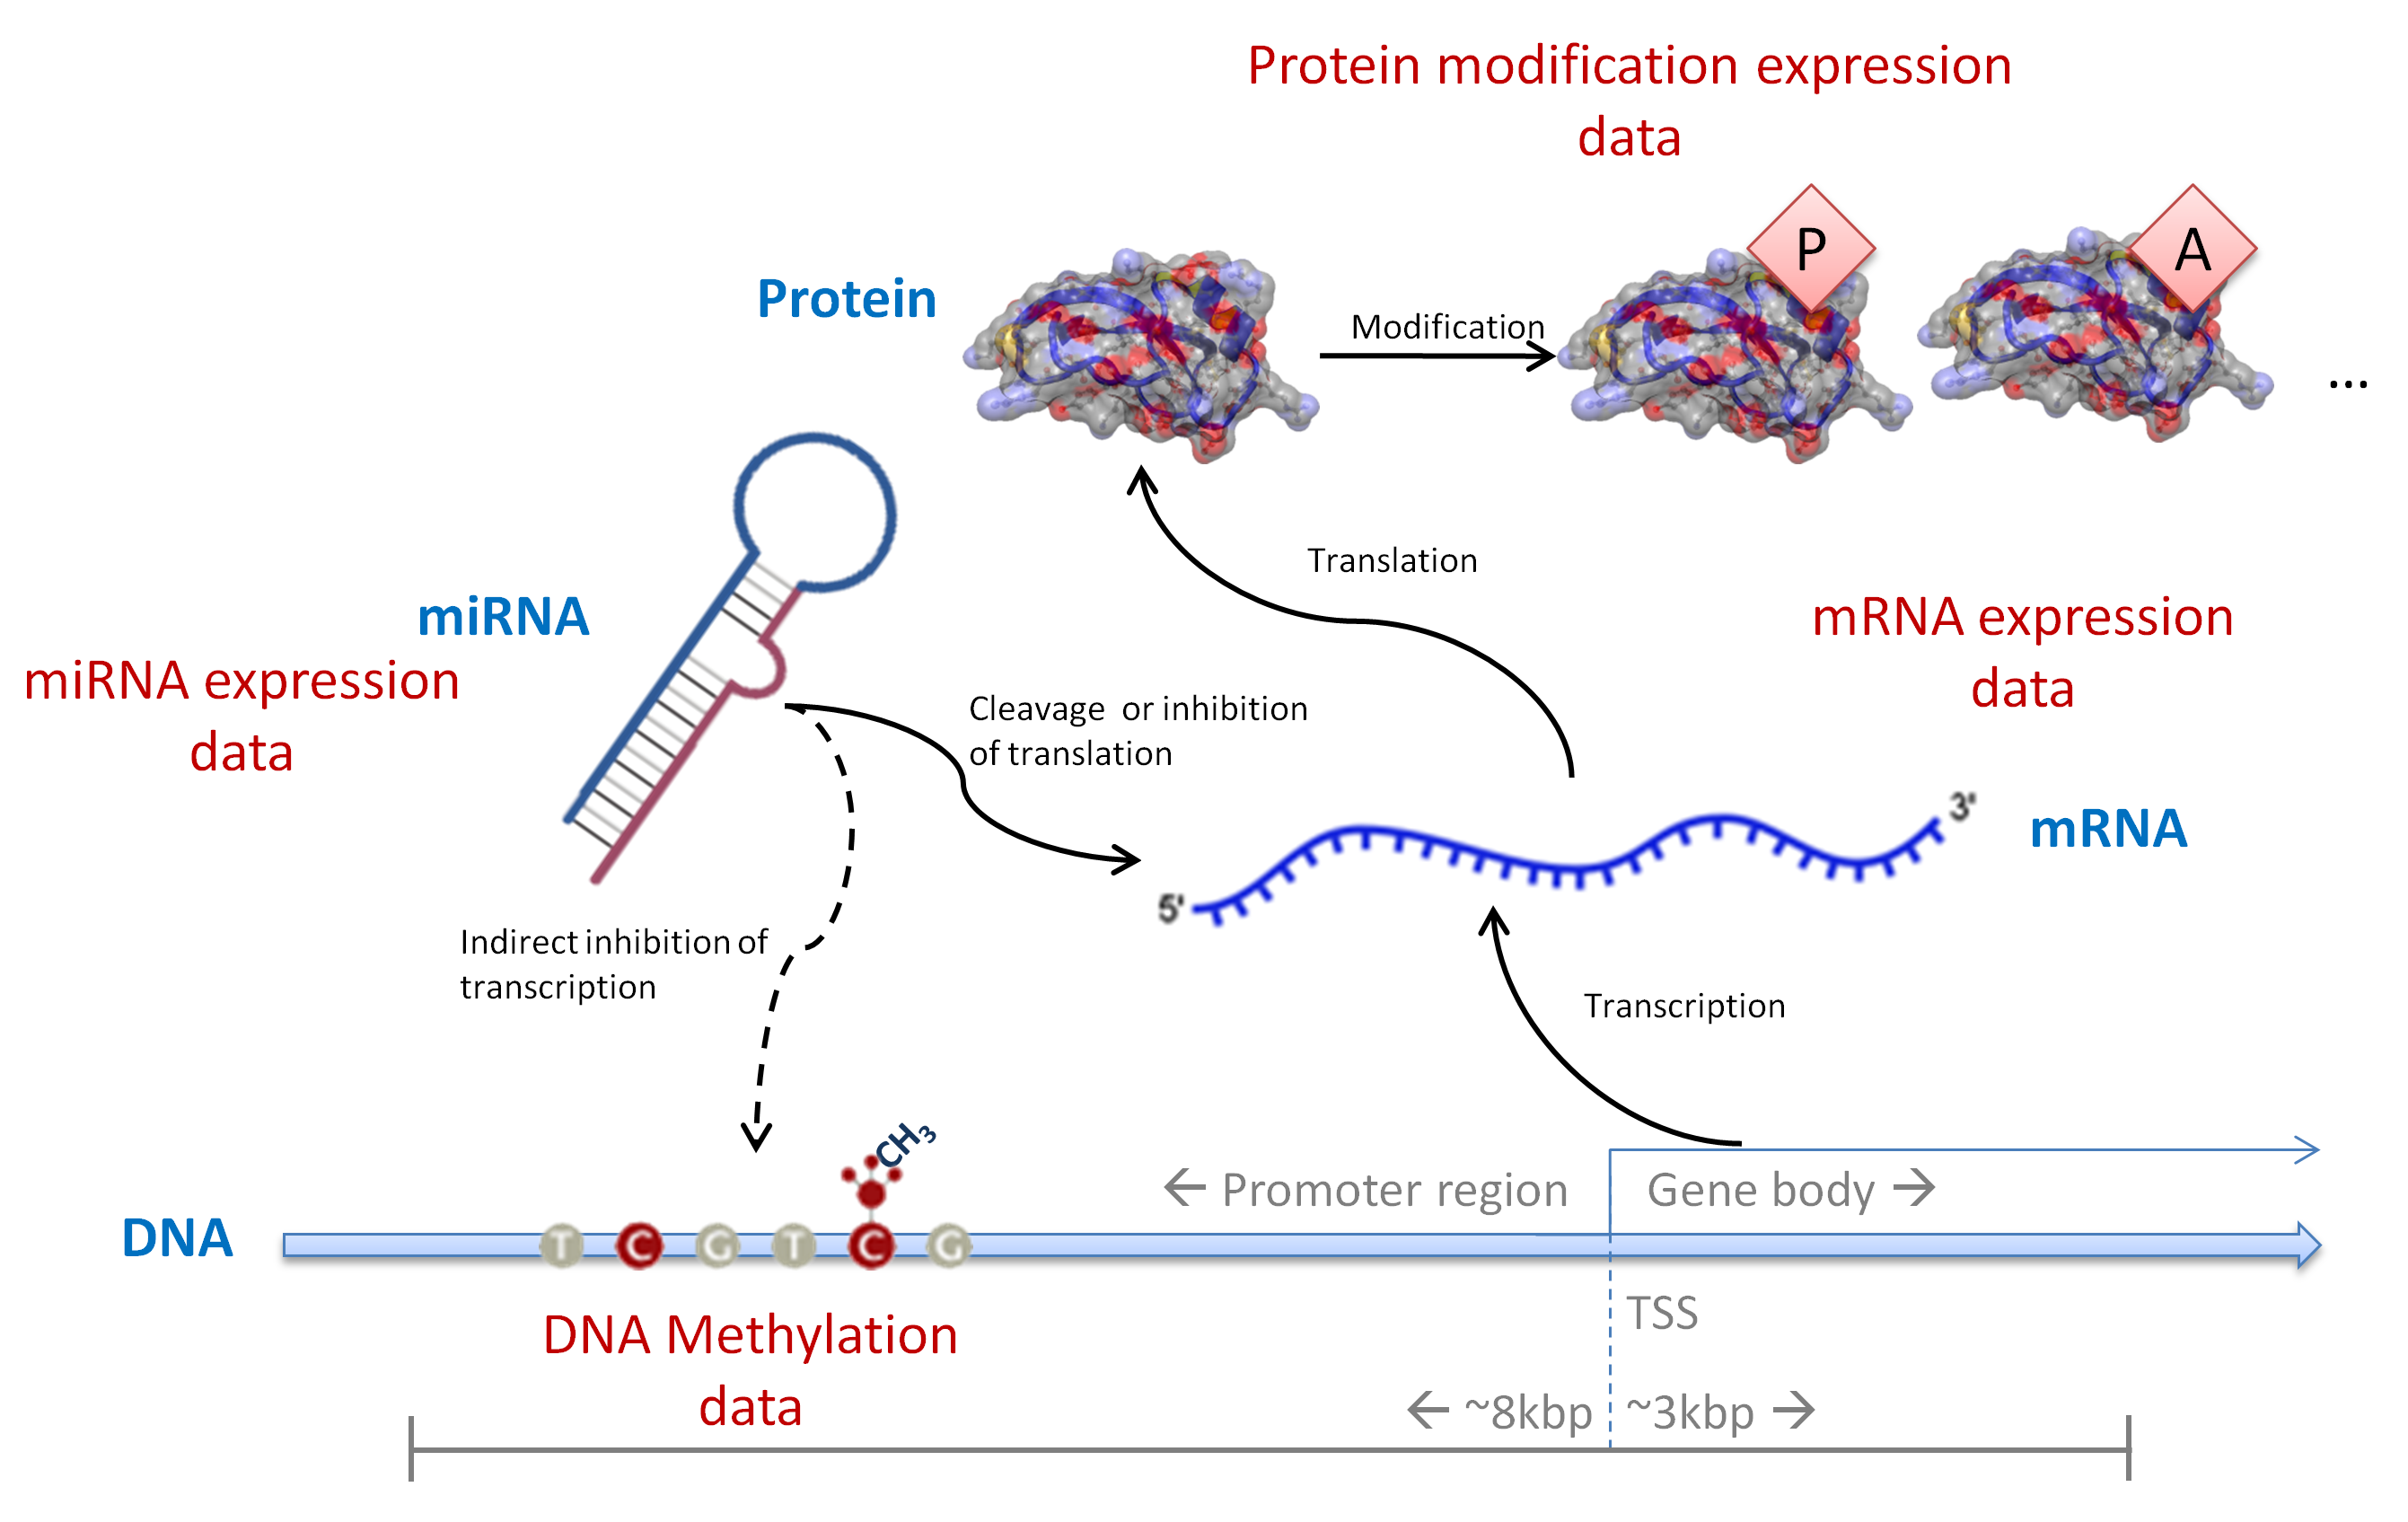
\includegraphics[width=1.0\textwidth]{figures/IntegratedDataAnalysis.png}
  \end{center}

\caption{
%{\bf Visualization of diverse microarray platforms that have been employed to perform an integrated data analysis.}
{\bf Visualization of different genomic and regulatory layers for which we propose cross-platform analysis and visualization methods.}
%
At the bottom of the figure, a DNA sequence is depicted for which methylation data is available. This DNA is transcribed to an mRNA. The transcription might be regulated by methylated regions on the gene promoter. Furthermore, miRNAs might inhibit the translation from mRNA to a protein. Both, mRNA and miRNA expression can be measured with microarrays. In the end, translated proteins might get modified, e.g., by phosphorylation or acetylation. The expression of basic proteins and specific modifications can be determined, e.g., by using reverse-phase protein arrays with several antibodies.
% Figure Caption from D4.1:
%Red fonts describe the actual data types and corresponding platforms. This figure is restricted to genomic interactions relevant for this deliverable. At the bottom of the figure, a DNA sequence is given, for which methylation data is available. This DNA is transcribed to an mRNA. The transcription might be regulated by methylated regions on the gene promoter. Furthermore, miRNAs might inhibit the translation from mRNA to a protein. Both, mRNA and miRNA expression is measured with Affymetrix and Agilent microarrays. In the end, translated proteins might get modified, e.g., by phosphorylation or acetylation. The expression of some basic isoforms and specific modifications is determined, using Zeptosens arrays.
}
\label{fig:1}
\end{figure}


%%%%%%%%%%%%%%%%%%%%%%%%%%%%%%%%%%%%%%
% Data Pairing
%%%%%%%%%%%%%%%%%%%%%%%%%%%%%%%%%%%%%%
\begin{figure}[!htb]
  \begin{center}
  %TODO: Convert to TIF (=> look at author guidelines)
    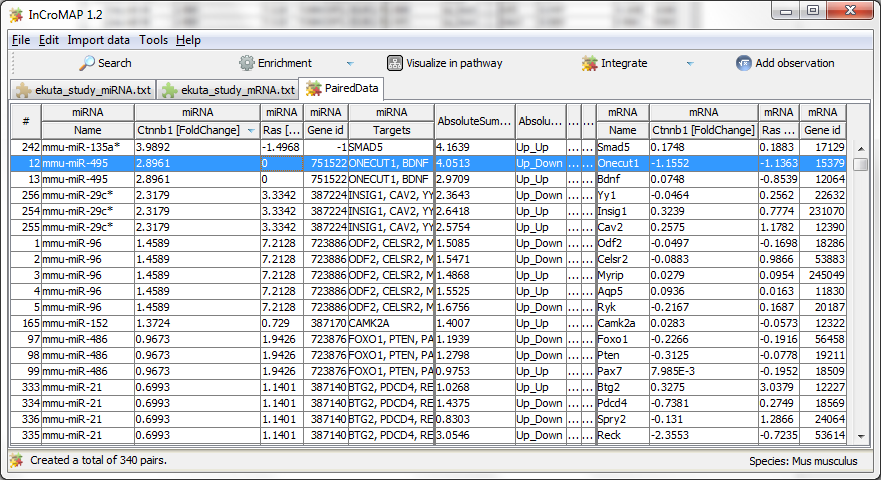
\includegraphics[width=1.0\textwidth]{figures/PairData-Onecut1Story.png}
  \end{center}

\caption{
{\bf Pairing of miRNA (left-hand side) and mRNA (right-hand side) datasets reveals miR-495 as a potential regulator of the HNF-6 coding gene \emph{Onecut1} in \emph{Ctnnb1}-mutated tumors.}
%\TODO{1 Caption �berarbeiten, 2 Ueberlegen ob Ras Expressionswerte ausgeblendet werden sollten und wenn nciht, "in Ctnnb1" in titel.}
Data pairing can be used to create a tabular representation of any two datasets. In this example, the effect of differentially expressed microRNAs on corresponding mRNA targets is visualized. The left-hand part of the table shows the miRNA data, sorted descending by log$_2$ fold change expression in \emph{Ctnnb1}-mutated tumors. The right-hand side of the table shows the targeted mRNAs, together with their fold change. Between both parts, some convenient information is shown, i.e., the absolute sum of miRNA and target mRNA fold changes in \emph{Ctnnb1}-mutated tumors and a textual representation of miRNA and corresponding mRNA expression.
%
This table shows that miR-495 is up-regulated and the corresponding mRNA target, \emph{Onecut1}, is down-regulated.
}
\label{fig:2:pairing}
\end{figure}


%%%%%%%%%%%%%%%%%%%%%%%%%%%%%%%%%%%%%%
% Multiple Integration
%%%%%%%%%%%%%%%%%%%%%%%%%%%%%%%%%%%%%%
\begin{figure}[!htb]
  \begin{center}
  %TODO: Convert to TIF (=> look at author guidelines)
    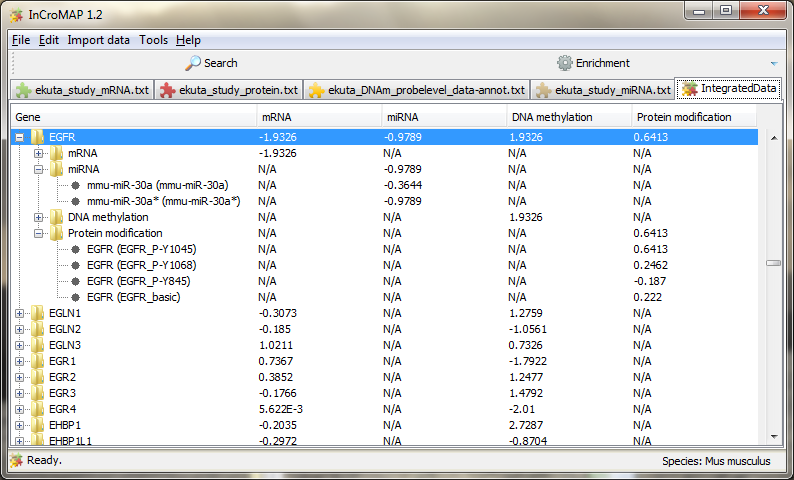
\includegraphics[width=1.0\textwidth]{figures/MultipleIntegrationEGFR.png}
  \end{center}

\caption{
{\bf Multiple integration of four different platforms from \emph{Ctnnb1} mutated tumors shows an mRNA decrease of \emph{Egfr} as a potential effect of DNA methylation increase in the promoter region.}
This tabular visualization integrates data from four different platforms in an expandable, gene-based manner. On the first layer, each row corresponds to one gene and each column to one platform. A summary value is displayed for each gene and platform. If expanded, the second layer shows different groups for mRNA, miRNA, DNA methylation and protein modification data. If these are further expanded, the single probes, miRNAs targeting this mRNA or protein modifications are shown, together with the corresponding expression fold change.
`N/A' indicates either `not applicable', e.g., the protein expression value for an mRNA probe, or `data not available'.
%
This tabular cross-platform integration of log$_2$ fold-changes shows that the promoter region of \emph{Egfr} has a maximum DNA methylation peak of $1.93$ and a minimum mRNA expression of $-1.93$. The mRNA is the target of two microRNAs and next to the basic protein, the expression of three different phosphoforms has been measured. A subsequent analysis of DNA methylation in the promoter region of \emph{Egfr} is depicted in Figure~\ref{fig:4:egfrMethylation}.
}
\label{fig:3:multipleIntegration}
\end{figure}


%%%%%%%%%%%%%%%%%%%%%%%%%%%%%%%%%%%%%%
% EGFR Methylation
%%%%%%%%%%%%%%%%%%%%%%%%%%%%%%%%%%%%%%
\begin{figure}[!htb]
  \begin{center}
  %TODO: Convert to TIF (=> look at author guidelines)
    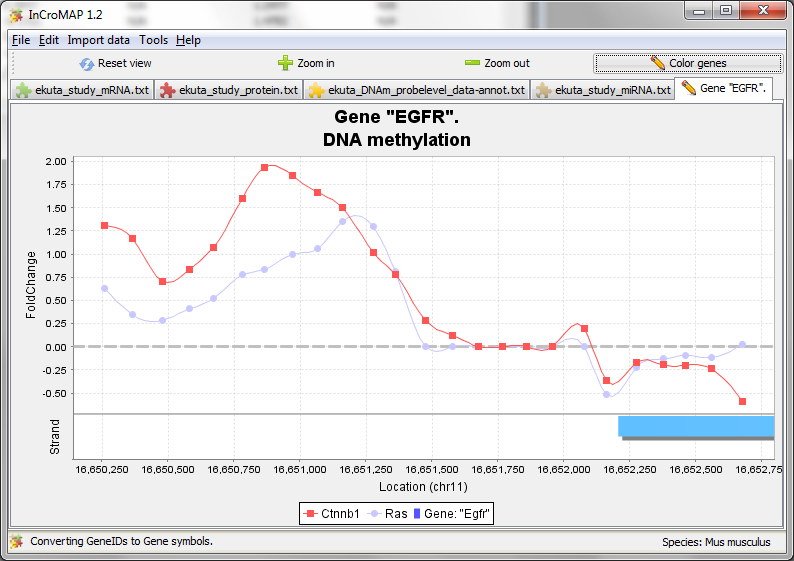
\includegraphics[width=1.0\textwidth]{figures/EGFR_methylation.png}
  \end{center}

\caption{
{\bf DNA methylation in the promoter region of \emph{Egfr} in \emph{Ctnnb1}-mutated tumors.}
This picture depicts the DNA methylation and mRNA expression changes for a region surrounding the transcription start site of \emph{Egfr} by $-2,000$ and $+500$\,bps. For DNA methylation, the fold changes of all probes in this region are visualized and connected by a curve. The gene body of \emph{Egfr} is depicted on the forward strand with a big box on the lower part of the picture. The blue-color indicates the mRNA expression of \emph{Egfr} in \emph{Ctnnb1}-mutated tumors (blue means down-regulation, red would indicate an up-regulation and color saturation denotes the intensity of the differential expression).
%In this example, the mRNA has an average log$_2$ fold change of -0.93.
In this example, the mRNA has a maximum differential log$_2$ fold change of $-1.93$.
}
\label{fig:4:egfrMethylation}
\end{figure}


%%%%%%%%%%%%%%%%%%%%%%%%%%%%%%%%%%%%%%
% Integrated enrichment
%%%%%%%%%%%%%%%%%%%%%%%%%%%%%%%%%%%%%%
\begin{figure}[!htb]
  \begin{center}
  %TODO: Convert to TIF (=> look at author guidelines)
  % Source Powerpoint file: "2011-09-20 IntegratedDataAnalysis-Flowchart".
    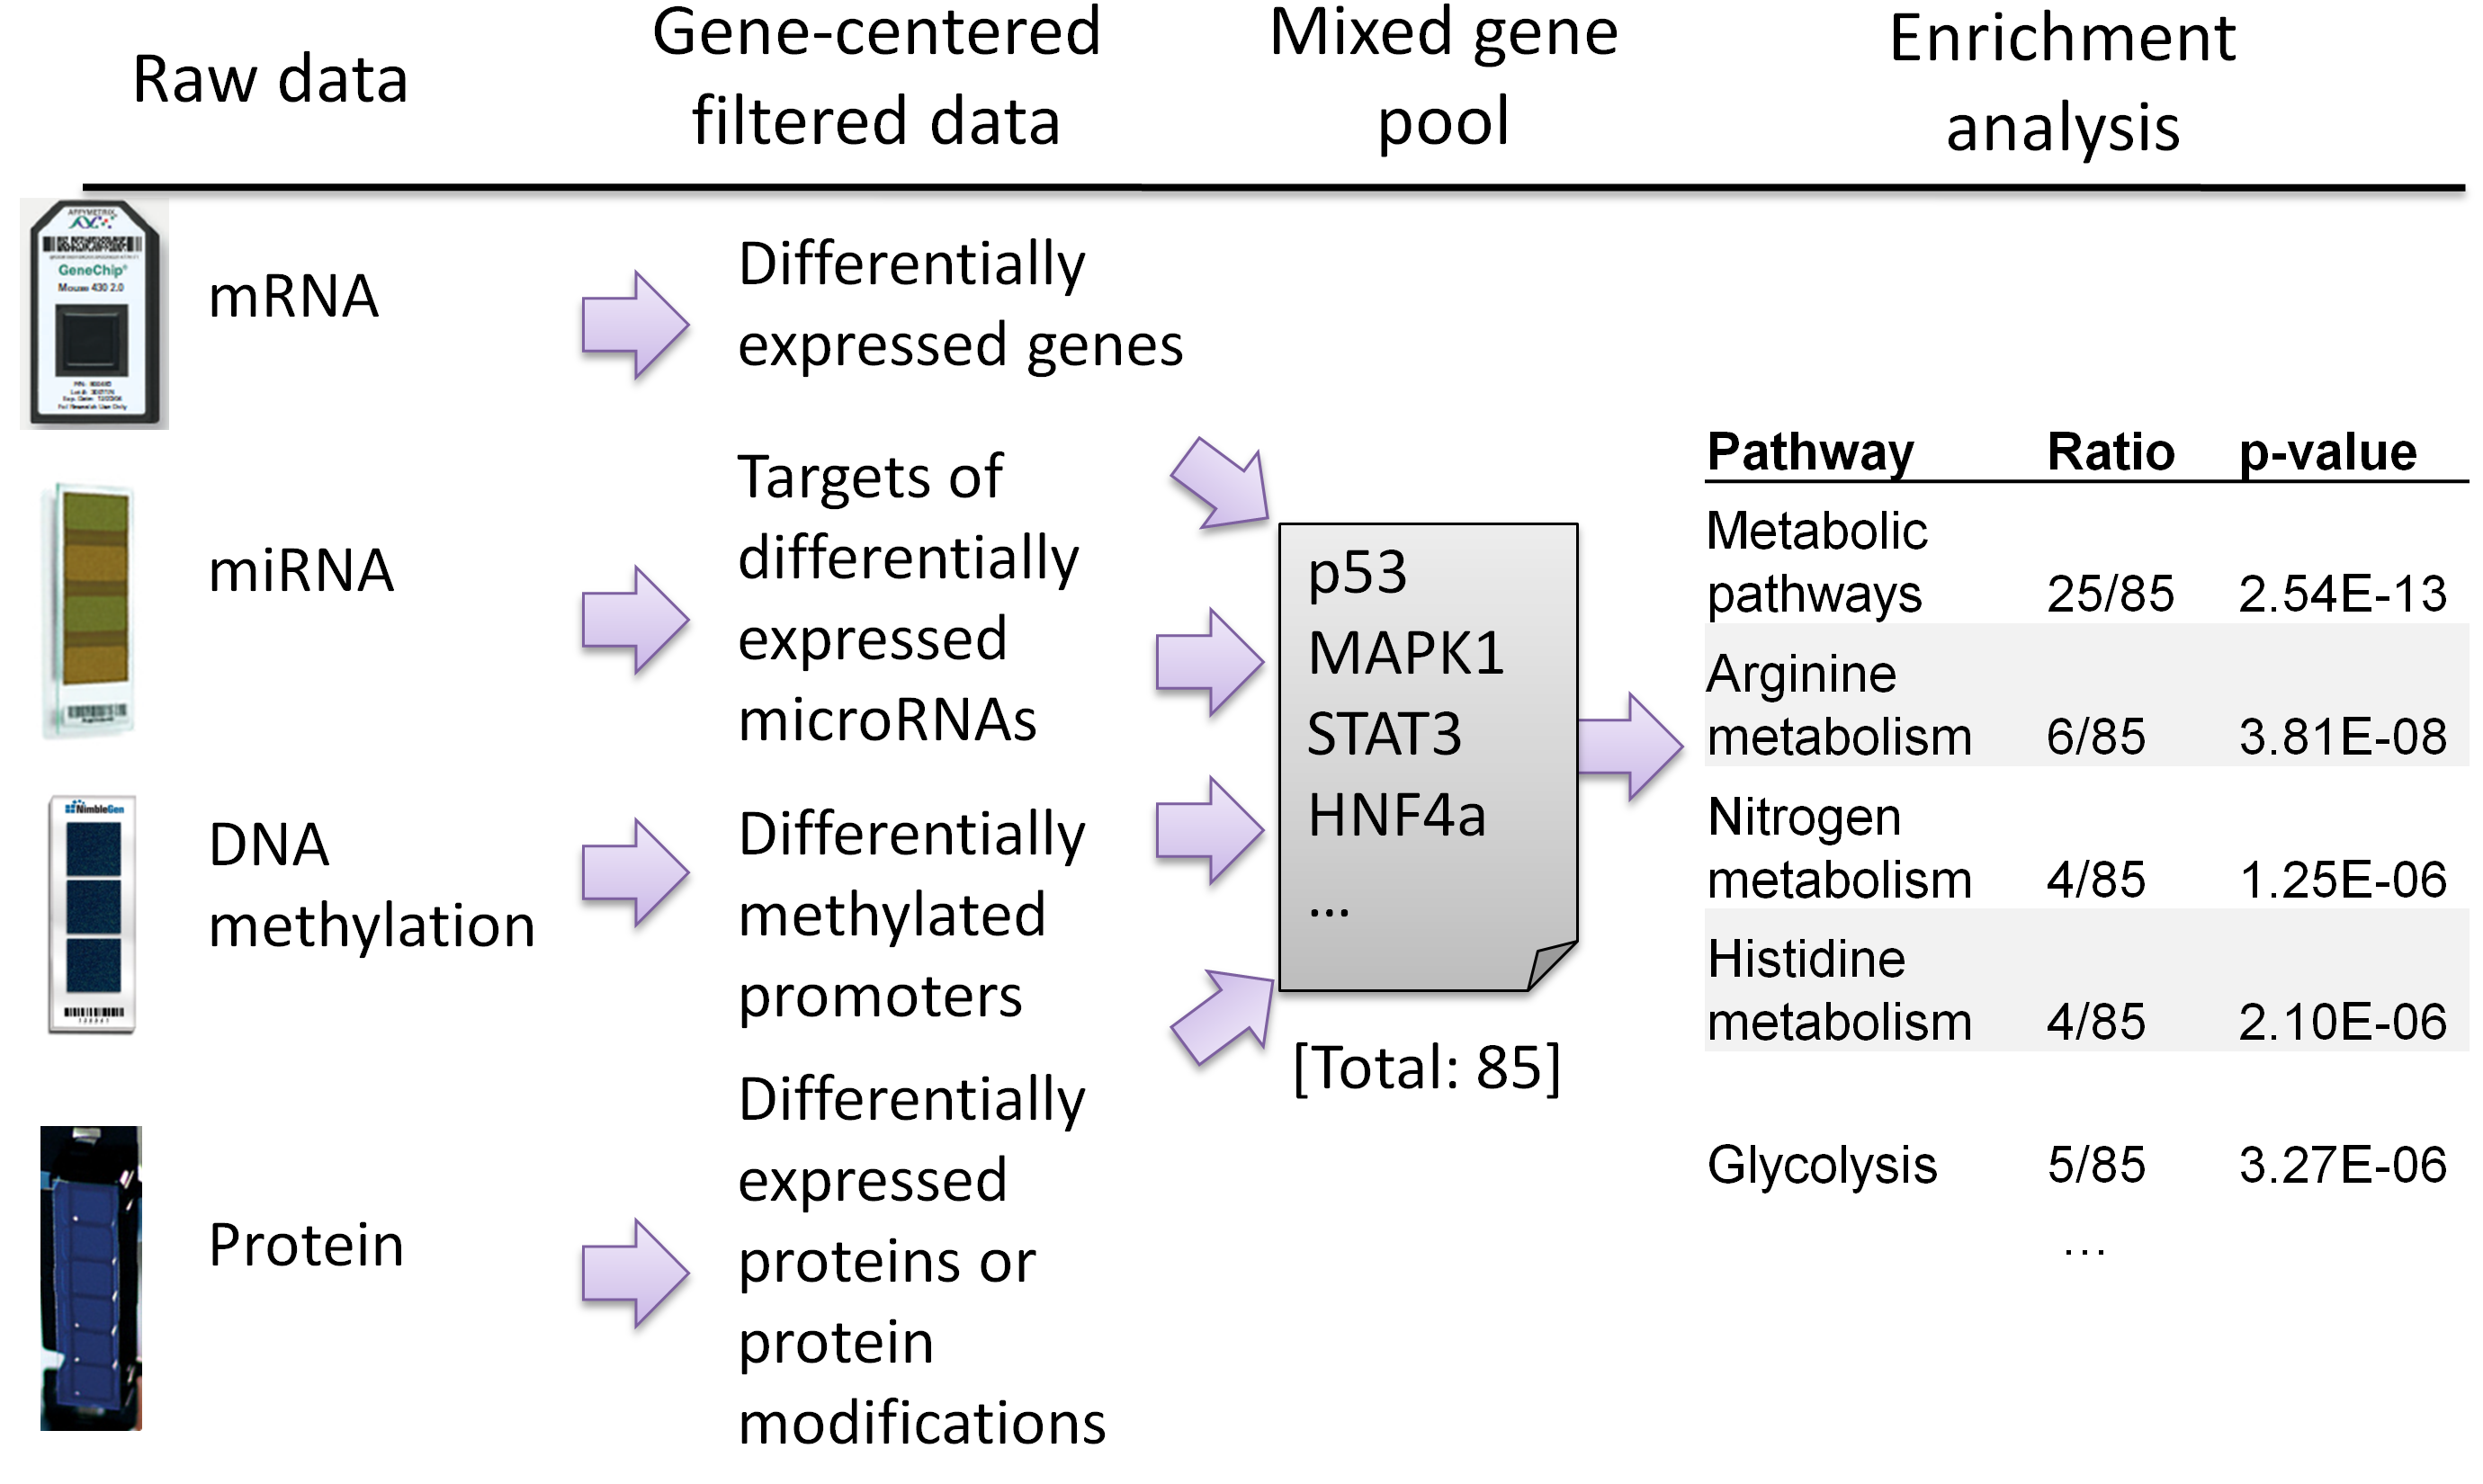
\includegraphics[width=1.0\textwidth]{figures/iEnrichment.png}
  \end{center}

\caption{
{\bf Proposed procedure for a cross-platform gene-set enrichment analysis.}
%\TODO{Bildunterschrift, 2 sagen dass 85 usw. examples sind.}
This flowchart depicts the major steps, involved in the creation of an integrated enrichment. The first two steps involve the evaluation of different datasets and extracting genes with strong platform-based changes as opposed to their corresponding control. In the third step, a mixed gene pool is created by joining all those gene lists (in this example, the result is a list of 85 genes). Finally, an enrichment is performed by comparing this list of genes to predefined gene sets and calculating a p-value, e.g., by using a hypergeometric distribution (see Subramanian \emph{et al.} for more information\cite{Subramanian2005}).
}
\label{fig:5:iEnrichment}
\end{figure}


%%%%%%%%%%%%%%%%%%%%%%%%%%%%%%%%%%%%%%
% Integrated enrichment vs. mRNA enrichment
%%%%%%%%%%%%%%%%%%%%%%%%%%%%%%%%%%%%%%
\begin{figure}[!htb]
  \begin{center}
  %TODO: Convert to TIF (=> look at author guidelines)
    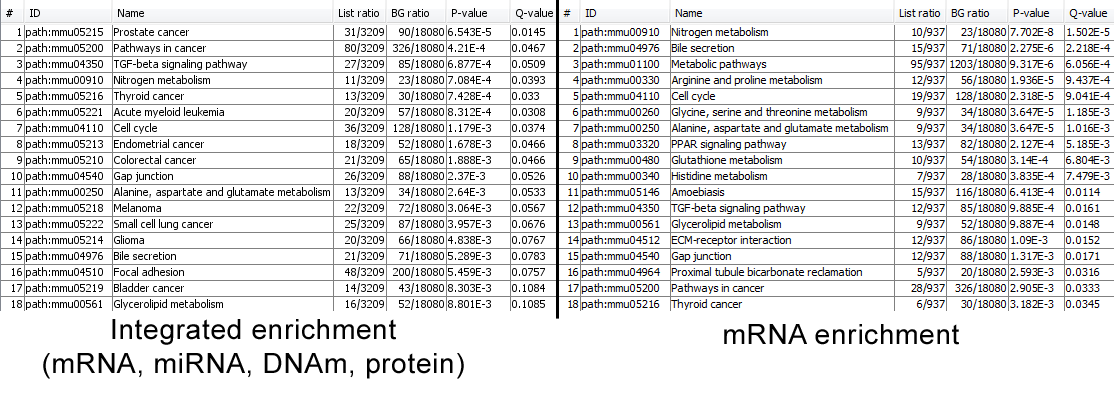
\includegraphics[width=1.0\textwidth]{figures/EnrichmentComparison_cut.png}
  \end{center}

\caption{
{\bf Comparison of an integrated and mRNA enrichment, based on data from \emph{Ctnnb1}-mutated tumors.}
%\TODO{Bildunterschrift, Metabolic vs. Cancer}
This comparison shows the difference between a KEGG pathway enrichment that is based only on mRNA data (right-hand side) and the result of an integrated enrichment (left-hand side). The integrated enrichment includes genes with differentially expressed mRNA, targets of differentially expressed microRNAs, differently expressed protein or protein modifications and genes with strong DNA methylation changes in their promoters.
It is clearly visible that the integrated enrichment provides a much broader insight into the pathway-changes in a tumor than using only a single dataset: Many cancer-related pathways are significantly impaired in the integrated enrichment, whereas the mRNA enrichment lists mainly metabolic pathways, which does only reflect the transcriptional changes.
}
\label{fig:6:iEnrichmentVsMRNA}
\end{figure}


%%%%%%%%%%%%%%%%%%%%%%%%%%%%%%%%%%%%%%
% Metabolic pathways overview map
%%%%%%%%%%%%%%%%%%%%%%%%%%%%%%%%%%%%%%
\begin{figure}[!htb]
  \begin{center}
  %TODO: Convert to TIF (=> look at author guidelines)
  %TODO: Add full image (+mRNA coloring) as supplementary material
    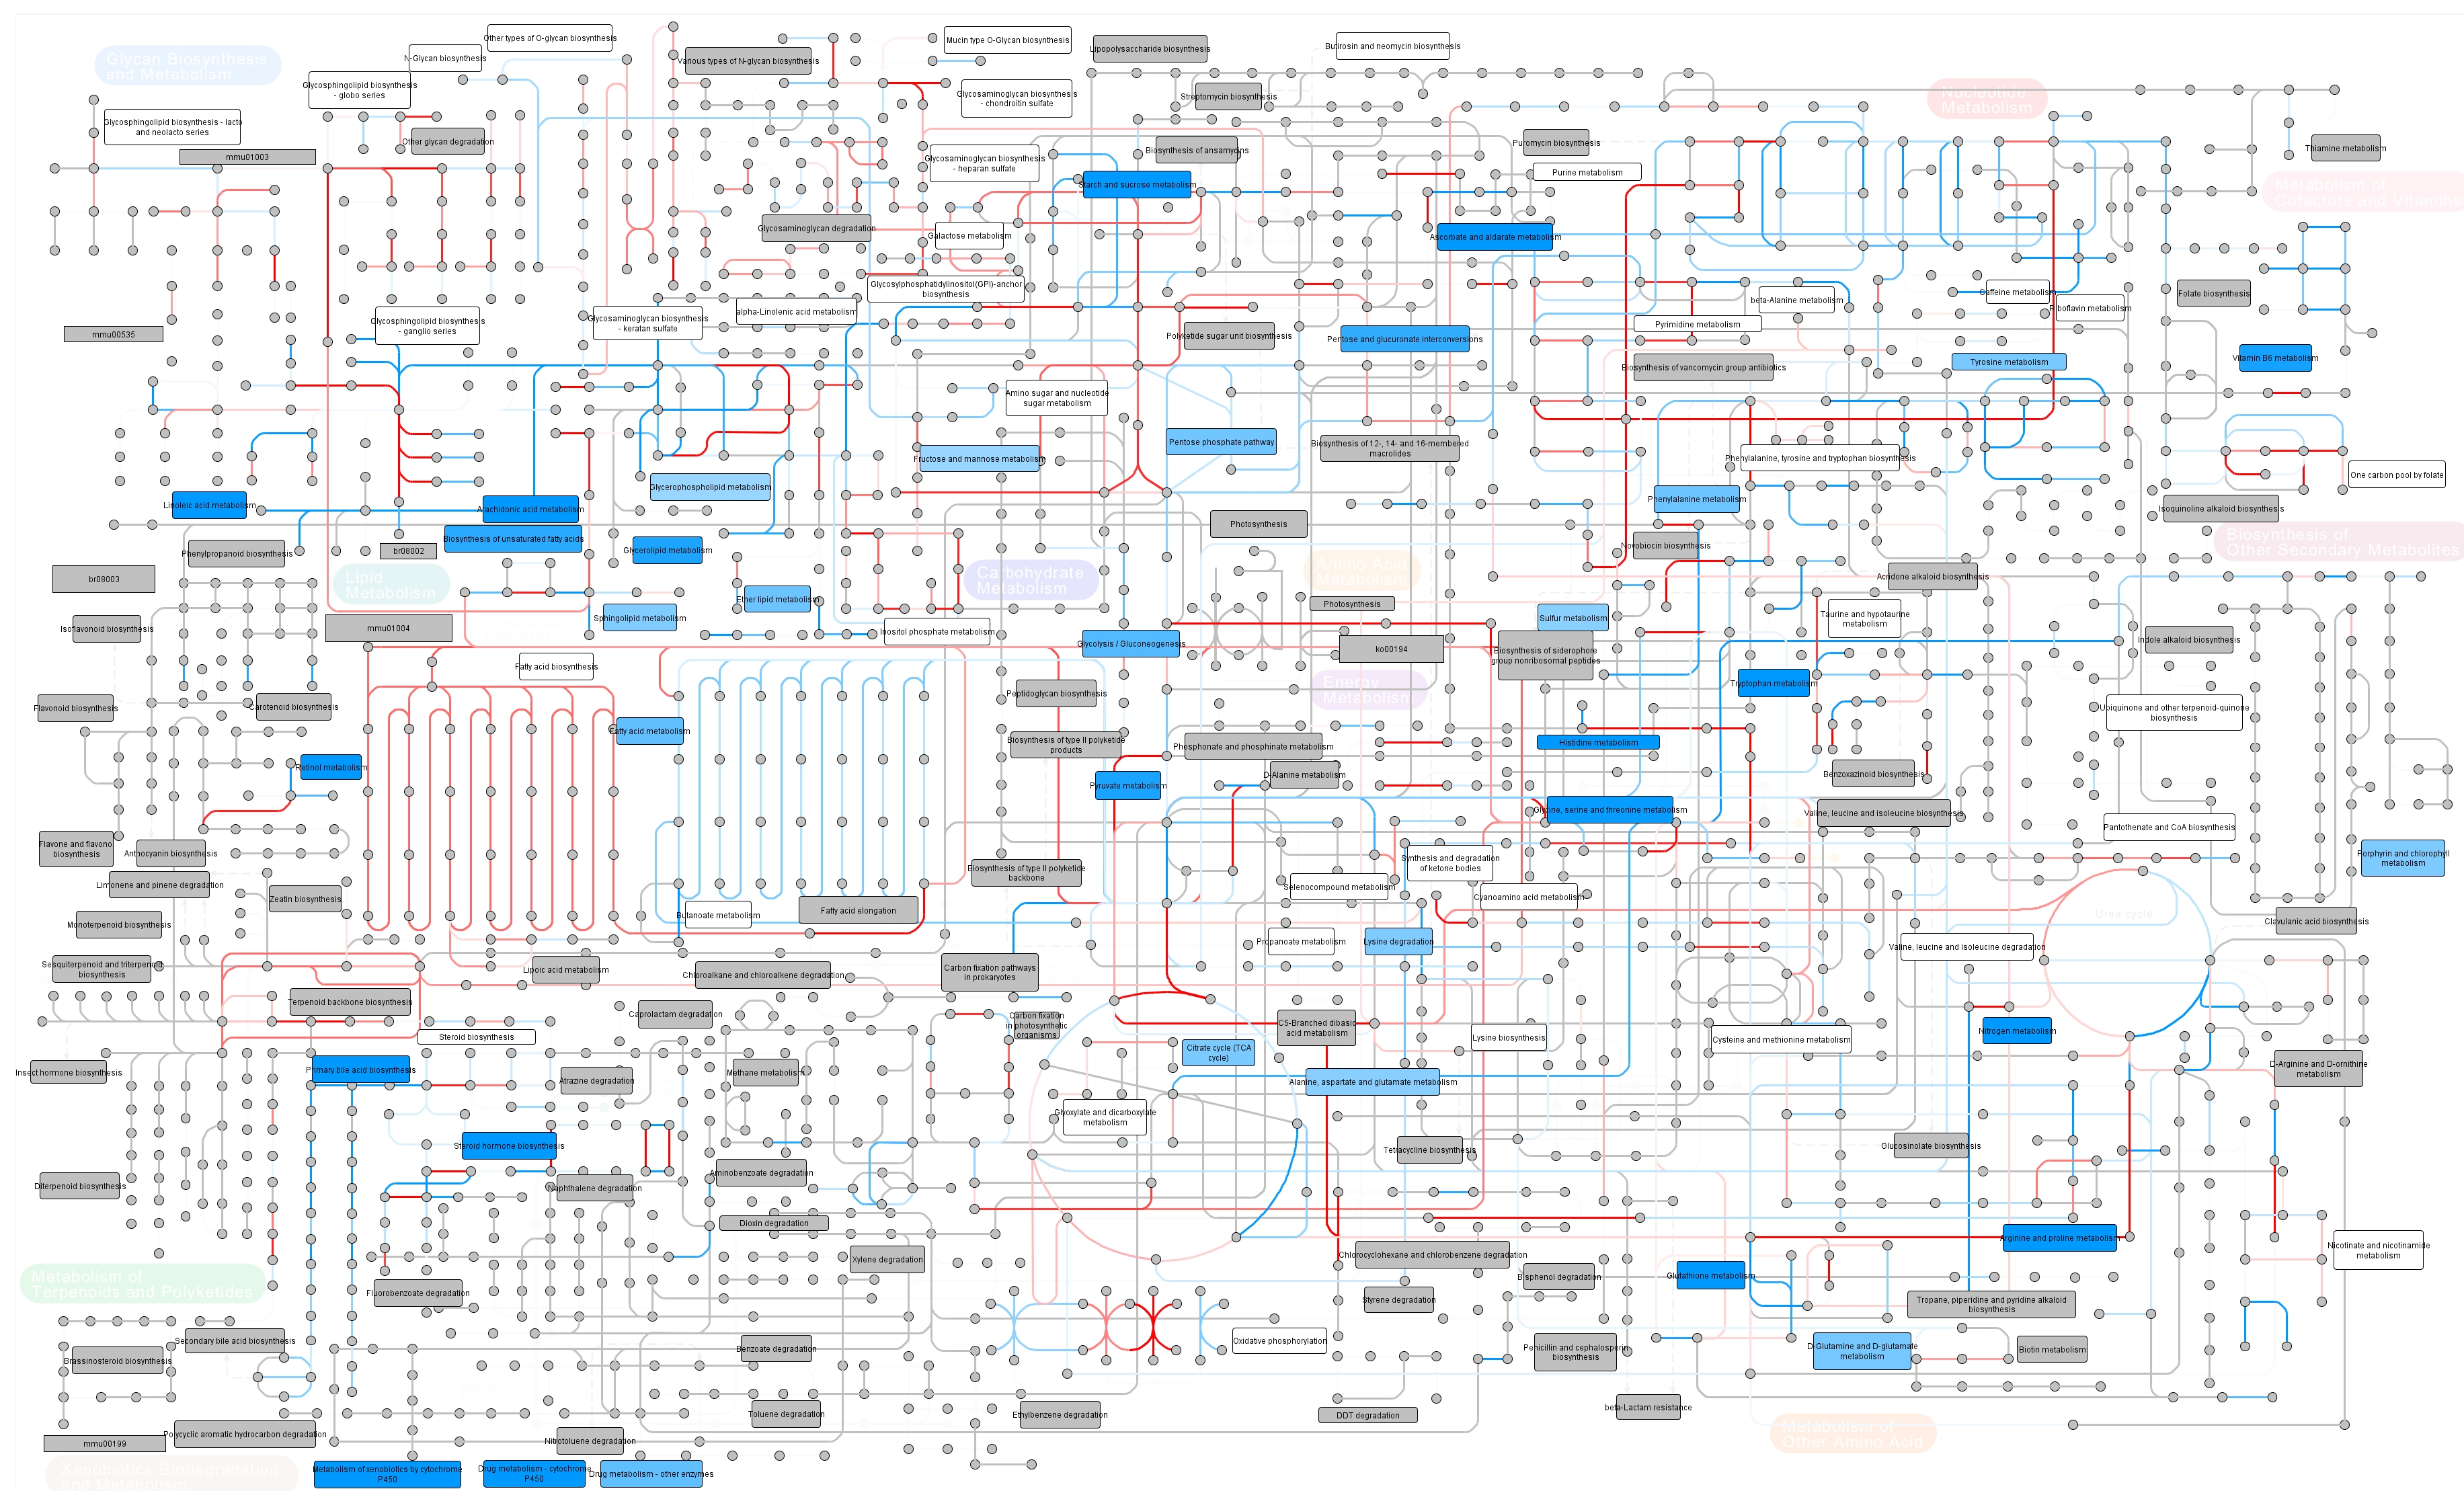
\includegraphics[width=1.0\textwidth]{figures/mmu01100_Ras_vs_Cat_noCPDlabels.jpeg}
  \end{center}

\caption{
{\bf Overview of transcriptional metabolic changes in \emph{Ha-ras}- and \emph{Ctnnb1}-mutated tumors.}
This visualization unifies pathway information, gene-set enrichment results and mRNA expression data to a single metabolic overview picture.
It is based on the mRNA differences between \emph{Ha-ras}- and \emph{Ctnnb1}-mutated tumors.
Compounds are depicted by grey circles and edges between them represent different enzymes. These edges are colored red, if the corresponding mRNA is higher expressed in \emph{Ha-ras}-mutated tumors and blue, if the corresponding mRNA is higher expressed in \emph{Ctnnb1}-mutated tumors. Grey indicates no differential expression. The bigger rectangles are references to other KEGG pathways and have been colored by significance (p-value) as a result of a pathway enrichment on the fold change differences between \emph{Ha-ras}- and \emph{Ctnnb1}-mutated tumors: A more saturated blue color indicates a lower p-value, white indicates p-values $>$ 0.05 and grey is used if no differential expression between both tumor types has been observed in the respective pathway. You can find a full-sized version of this picture in the supplement.
%
%\TODO{Bildunterschrift, 2 Integrates a) pathway b) enrichment c) (on mRNA). 3 Can be extended to line-color mRNA 4 Volles Bild + mRNA kanten im supplement}
%\TODO{\newline Was sollten wir hier genau zeigen?
%\newline-- Gesamtes Bild oder bestimmter Ausschnitt? Wenn Ausschnitt, welcher?
%\newline-- Kanten nach mRNA einfaerben oder nicht?
%\newline-- Compound Beschriftungen verstecken oder zeigen? (Derzeit sind sie nicht beschriftet!)
%}
}
\label{fig:7:metabolicOverview}
\end{figure}


%%%%%%%%%%%%%%%%%%%%%%%%%%%%%%%%%%%%%%
% Single platform in pathway visualization explanation
%%%%%%%%%%%%%%%%%%%%%%%%%%%%%%%%%%%%%%
\begin{figure}[!htb]
  \begin{center}
  %TODO: Convert to TIF (=> look at author guidelines)
    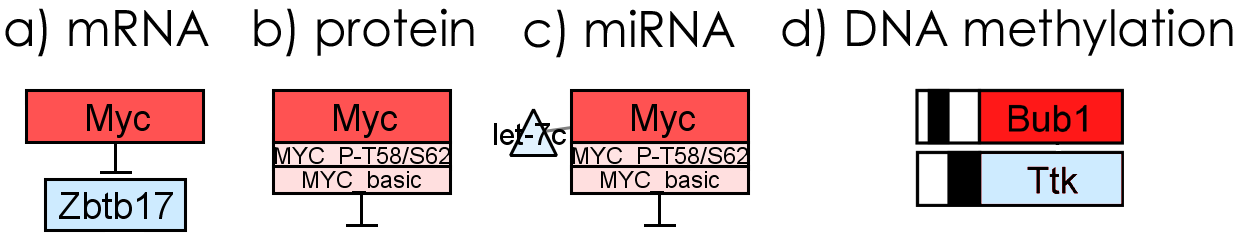
\includegraphics[width=1.0\textwidth]{figures/Platform_visualization.png}
  \end{center}

\caption{
{\bf Pathway-based visualization of different platforms.}
This figure shows how data from different platforms can be jointly visualized in a pathway. A) Messenger RNA expression changes are visualized as node color. Red is used to indicate up-regulation, blue is used for down-regulation and white indicates no differential expression (i.e., fold-change is zero). More saturated colors indicate stronger differential expression. B) Protein modification data is visualized by adding small boxes below the node. In this example, one box is used for the basic protein and one for a phosphorylated isoform. `MYC P-T58/S62' indicates an antibody that detects changes specifically for MYC proteins that are phosphorylated on Threonine 58 and Serine 62.
The color scheme is the same as for the mRNA. C) MicroRNAs are added to pathways as small triangles that are connected to their potential mRNA targets. MicroRNA expression data is then visualized by changing to color of the microRNA as described above. D) DNA methylation data is summarized by taking the maximum differential peak in the corresponding gene promoter. This peak is visualized by a black bar that stretches from the middle to the left to indicate hypomethylation and from the middle to the right to indicate hypermethylation. In the depicted examples, \emph{Bub1} shows a hypomethylation (log$_2$ fold change of approximately 1) and \emph{Ttk} shows a strong hypermethylation (log$_2$ fold change of $\geq$ 1.5).
Figure~\ref{fig:10:WNTCtnnb1} shows an example in which all four visualization techniques are used to create a joint pathway-based visualization of data from heterogenous platforms.
}
\label{fig:8:pwVisPlatformsExplanation}
\end{figure}


%%%%%%%%%%%%%%%%%%%%%%%%%%%%%%%%%%%%%%
% Glycolysis mRNA/DNAm Ctnnb1/Ha-Ras Comparison
%%%%%%%%%%%%%%%%%%%%%%%%%%%%%%%%%%%%%%
\begin{figure}[!htb]
  \begin{center}
  %TODO: Convert to TIF (=> look at author guidelines)
  % Source Powerpoint file: "Glycolysis".
    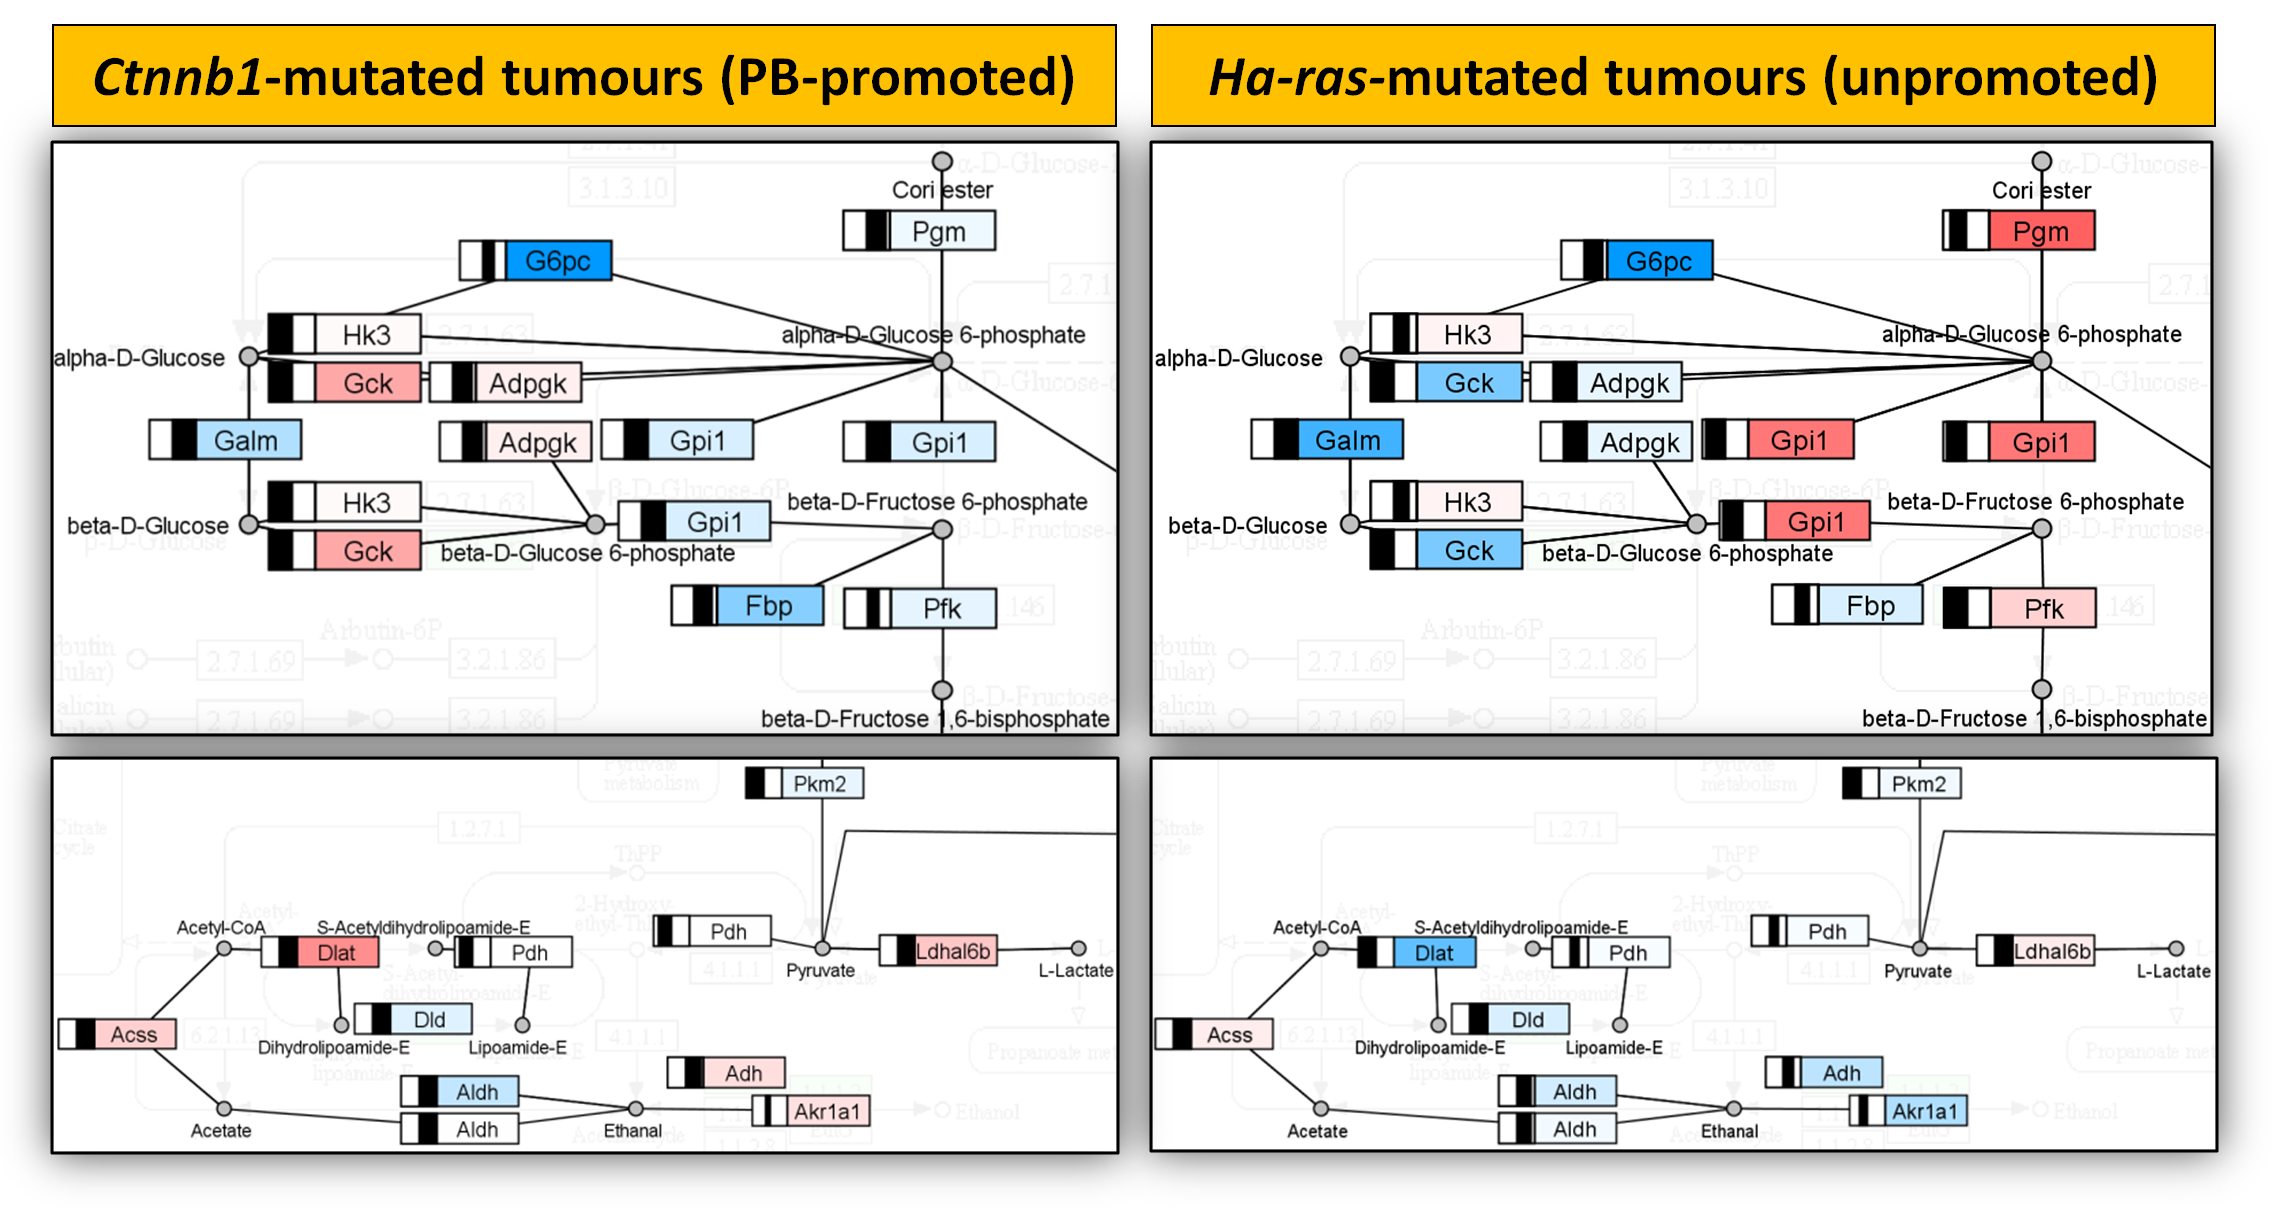
\includegraphics[width=1.0\textwidth]{figures/Glycolysis.png}
  \end{center}

\caption{
{\bf Integrated view of transcriptional and epigenetic changes in parts of the Glycolysis/ Gluconeogenesis pathway during profiling of \emph{Ha-Ras} and \emph{Ctnnb1} mutated tumors.}
%
The pictures on the left show mRNA and DNA methylation changes in the \emph{Ctnnb1}-mutated tumors, which is mediated by phenobarbital (PB). For comparison, the same parts of the pathway are visualized on the right-hand side with data from \emph{Ha-ras}-mutated tumors, which were not treated with PB.
%
Briefly, nodes are colored according to mRNA expression changes (red means up-regulation and blue means down-regulation) and the black bar left of each node indicates DNA methylation changes (please see Figure~\ref{fig:8:pwVisPlatformsExplanation} for a more detailed legend).
%
%
%%
%Glucokinase (Gck) -- katalysiert den 1. Schritt des Glucose-Abbaus in der Glykolyse: Genexpression hochreguliert, Promotorregion hypomethyliert.
%%
%Glucose-6-phosphatase (G6PC) -- katalysiert den der Gck entgegengesetzten Schritt in der Glukoneogenese, also dem Synthese von Glukose. Dieses Gen ist in beiden Tumortypen runterreguliert, dazu passt, dass die Promotorregion bei beiden weitestgehend hypermethyliert ist.
%%
%Fructose-1,6-bisphosphatase (FBP) -- auch ein Enzym der Gluconeogenese, in beiden Tumortypen runterreguliert mit hypermethylierter Promotorregion.
%%
%Bei Pgm, Aldo und anderen eingef�rbten Enzymen w�re ich pers�nlich jetzt noch vorsichtig mit irgendwelchen Aussagen, weil da oft nur sehr wenige Sonden gemessen wurden oder die Sonden widerspr�chliche Werte zeigen.
%%
%Korrelation von DNAm und mRNA ist teilweise recht interresant!
%%
}
\label{fig:9:GlycolysisCtnnb1Ras}
\end{figure}


%%%%%%%%%%%%%%%%%%%%%%%%%%%%%%%%%%%%%%
% WNT_signaling with four data types
%%%%%%%%%%%%%%%%%%%%%%%%%%%%%%%%%%%%%%
\begin{figure}[!htb]
  \begin{center}
  %TODO: Convert to TIF (=> look at author guidelines)
  % Source Powerpoint file: "Glycolysis".
    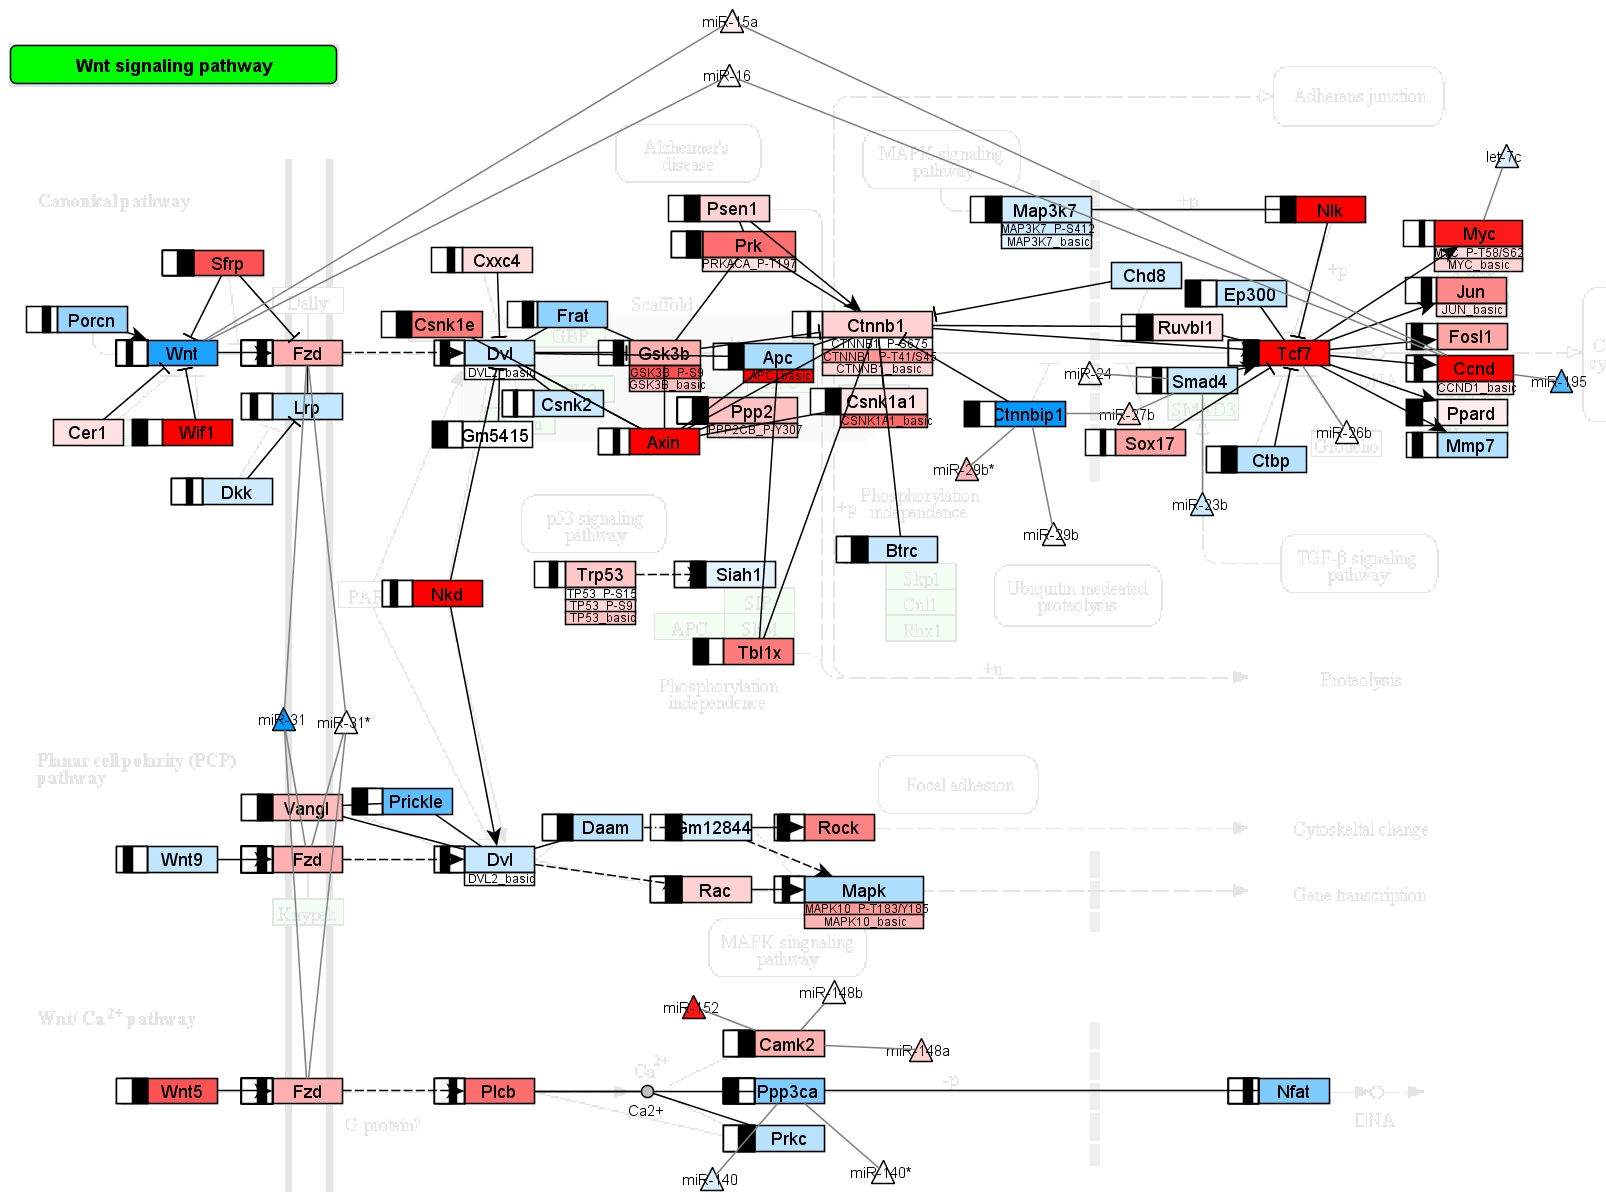
\includegraphics[width=1.0\textwidth]{figures/WNT_signaling.jpeg}
  \end{center}

\caption{
{\bf Integrated visualization of DNA methylation, protein modification, microRNA and messenger RNA changes in the WNT signaling pathway of \emph{Ctnnb1} mutated tumors.}
Characteristic perturbations in Ctnnb1 mutated tumors across multiple layers of gene-regulation are depicted in this picture. In general, red means up-regulation and blue means down-regulation. More saturated colors indicate stronger differential regulation. Messenger RNA expression is shown directly as node color, microRNAs are connected to their mRNA targets and colored according to microRNA expression and protein modification data is shown in small separate boxes below the actual nodes. DNA methylation is indicated with a black bar in a black surrounded box, ranging from the middle to the left to indicate hypomethylation and to the right to indicate hypermethylation.
%The up-regulated transcription factors \emph{Myc}, \emph{Jun}, \emph{Fosl1} and \emph{Ccnd1} constitute main targets of the pathway.
}
\label{fig:10:WNTCtnnb1}
\end{figure}

%\section*{Tables}
%\begin{table}[!ht]
%\caption{
%\bf{Table title}}
%\begin{tabular}{|c|c|c|}
%table information
%\end{tabular}
%\begin{flushleft}Table caption
%\end{flushleft}
%\label{tab:label}
% \end{table}

\end{document}

